\documentclass[9pt,twocolumn,twoside]{osajnl}
%% Please use 11pt if submitting to AOP
 %\documentclass[11pt,onecolumn,twoside]{osajnl}

\journal{josab} % Choose journal (ao, aop, josaa, josab, ol)
\graphicspath{{figures/}}
% See template introduction for guidance on setting shortarticle option
\setboolean{shortarticle}{false} 
% true = letter / tutorial 
% false = research / review article 
% (depending on journal).

\title{Modulating quantum fluctuations of scattered light in disordered media via wavefront shaping}

\author[1,2,*]{Dong Li}
\author[1,2,$\dagger$]{Yao Yao}

\affil[1]{Microsystems and Terahertz Research Center, China Academy of Engineering Physics,
Chengdu Sichuan 610200, P. R. China}
\affil[2]{Institute of Electronic Engineering, China Academy of Engineering Physics, Mianyang Sichuan 621999, P. R. China}


\affil[$\dagger$]{Corresponding author: yaoyao@mtrc.ac.cn}
\affil[*]{Corresponding author: lidong@mtrc.ac.cn}
%% To be edited by editor
% \dates{Compiled \today}

\ociscodes{(270.0270) Quantum optics; (170.7050) Turbid media; (270.6570) Squeezed states; (110.7348) Wavefront encoding.}

%% To be edited by editor
% \doi{\url{http://dx.doi.org/10.1364/XX.XX.XXXXXX}}

\begin{abstract}
After multiple scattering of quadrature-squeezed light in a disordered medium, the quadrature amplitudes of the scattered modes present an excess noise above the shot-noise level [P. Lodahl, Opt. Expr. 14, 6919 (2006)]. A natural question is raised whether there exists a method of suppressing the quadrature fluctuation of the output mode. The answer is affirmative. In this work, we prove that wavefront shaping is a promising method to reduce the averaged quantum noise of quadrature amplitudes of the scattered modes. This reduction is owing to the destructive interference of quantum noise. Specifically, when the single-mode squeezed states are considered as inputs, the averaged quantum fluctuation can always be reduced, even below the shot-noise level. These results may have potential applications in quantum information processing, for instance, sub-wavelength imaging using the scattering superlens with squeezed-state sources.
\end{abstract}

\setboolean{displaycopyright}{true}

\begin{document}

\maketitle

\section{Introduction}

The studies of nonclassical light illuminating a disordered medium have received increasing attentions in recent years \cite{b1998,smolka2009,peeters2010,Beenakker2000,lodahl2005a,lodahl2005b,patra1999,patra2000,two2002,wiersma2013,lahini2010,gilead2015,defienne2016,leonetti2013,starshynov2016,an2018,walschaers2016,zhang2018,vellekoop2010np,rotter2017,xu2017a,xu2017b}, which is due to the fact that this quantum optical system has significant implications for quantum information processing, including Heisenberg-limit resolution imaging \cite{hong2017,hong2018}, programmable quantum optical circuit \cite{wolterink2016,huisman2014,defienne2014}, quantum communication \cite{b2017}, and quantum optical authentication \cite{goorden2014,nikolopoulos2017,yao2016,li2017}. 

As a typical nonclassical state, the squeezed state is of importance because it can achieve lower quantum noise than the quantum fluctuation of coherent state (\textit{or} equivalently the shot noise) \cite{walls1983,walls2007,barnett2002,lvovsky2015}. As a consequence, the squeezed state can enhance signal-to-noise ratio \cite{caves81,yurke86,xiao1987precision} and has been utilized in different applications ranging from quantum imaging \cite{beskrovnyy2005,sokolov2004} to gravitational wave detection \cite{aasi2013,barsotti2018,mehmet2018}.

From the perspective of quantum theory of light, the multiple scattering of squeezed states in disordered media [Fig. \ref{fig1}(a)] is a question of general interest, which has been explored from different aspects recently. For example, Ott \textit{et al.} \cite{ott2010} investigated the pairwise entanglement of scattered beams in 2010. It was found that the entanglement can be induced by multiple scattering of the squeezed state. Recently, our previous work \cite{li2019} examined the statistical distribution of quantum correlation of the scattered modes. Lodahl \cite{lodahl2006b} studied the quantum fluctuation of scattered modes and found that the averaged quantum fluctuation of quadrature amplitudes of the scattered modes is always larger than the shot noise. 

Intriguingly, it is noteworthy that in Ref. \cite{lodahl2006b} the input is a single-mode squeezed state with a sub-shot noise whereas the output exhibits an excess noise [i.e. noise above the shot-noise level, (SNL)]. In other words, after multiple scattering, the mean quantum noise of the scattered modes becomes larger than the incident one. Since the large quantum noise is detrimental for precision detection, we wonder whether there exists a method to suppress the output quantum noise.
 

Actually, wavefront shaping (WFS) is an emerging technology for optical focusing and imaging through disordered media \cite{vellekoop2007,vellekoop2008,popoff2010,mosk2012}, by controlling the incident wavefront, which paves a way for manipulating the speckle pattern in a desired manner. In general, WFS can be performed by spatial light modulator (SLM) in experiments as depicted in Fig. \ref{fig1}(b). The SLM acting as a reprogrammable matrix of pixels imprints expected phase values, $\phi_n$, on the coherent wavefront. In recent decades, it has been extensively utilized in numerous optical applications, such as, quantum simulator \cite{prl2019}, quantum data locking \cite{lum2016}, and super-resolution imaging \cite{putten2011,park2014,jang2018,chen2018}.

\begin{figure*}[h]
\begin{center}
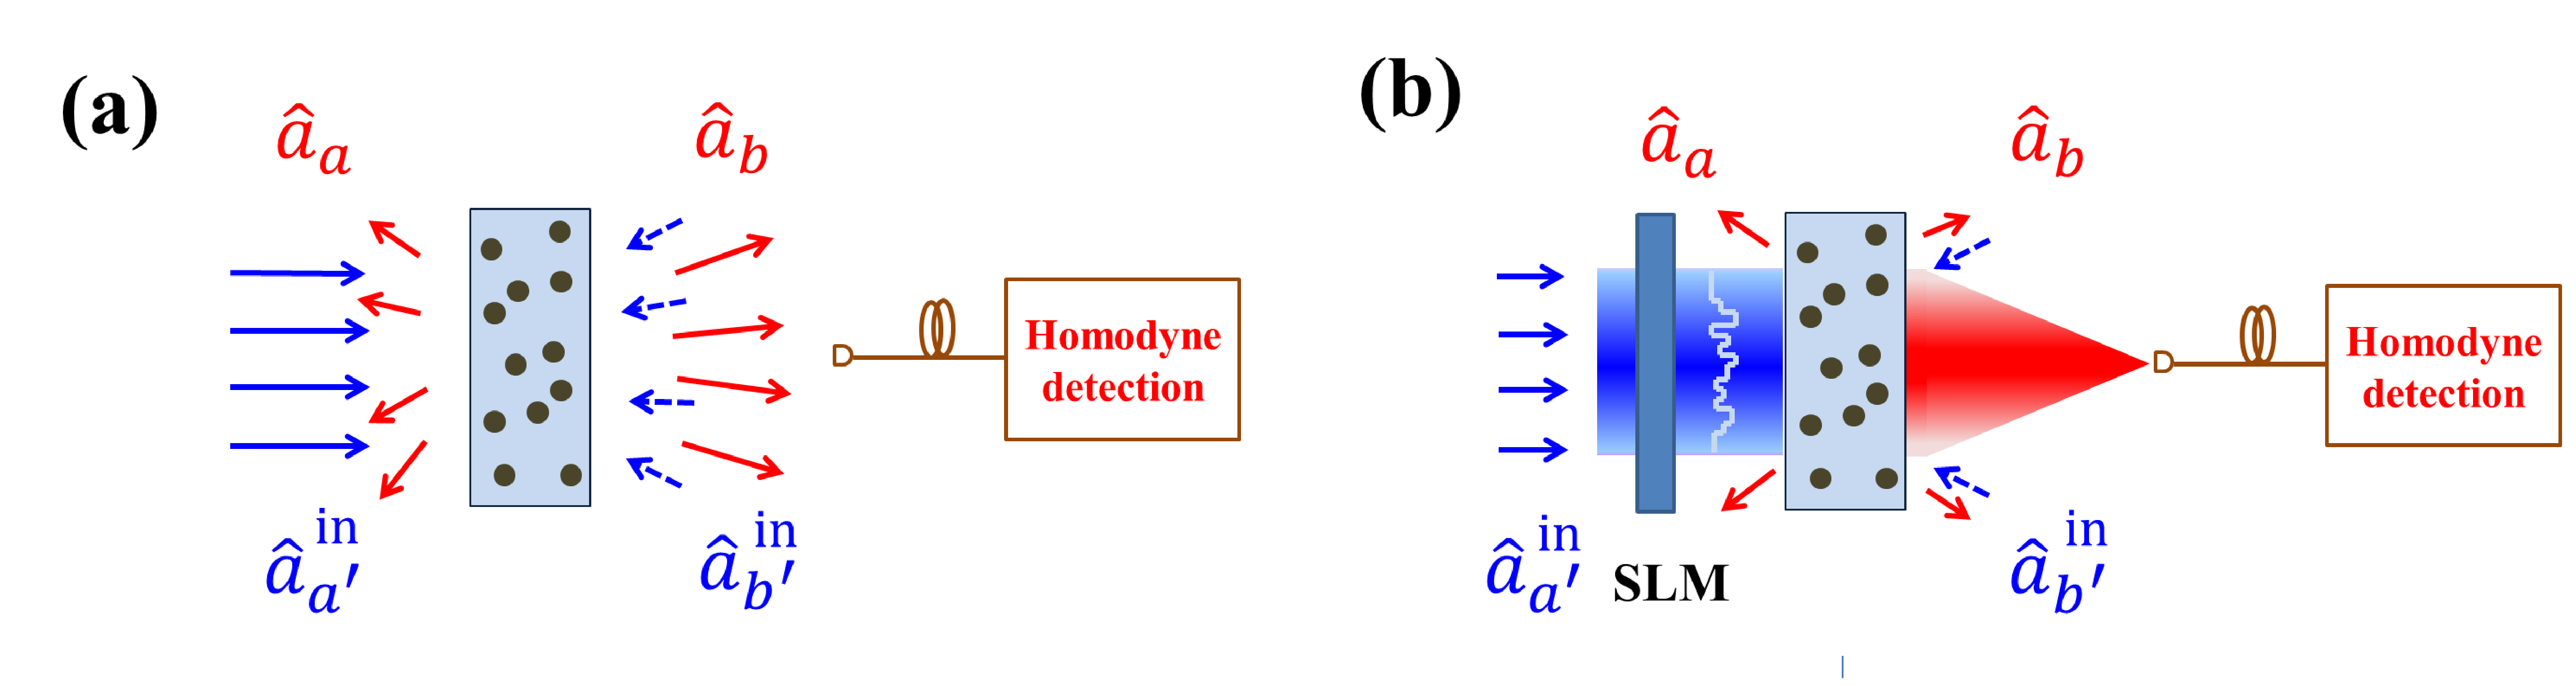
\includegraphics[width=.90\textwidth]{00_20190604_setup.eps} {}
\end{center}
\caption{Quadrature fluctuation detections of beams transmitted through a disordered medium (a) in the absence of WFS, (b) in the presence of WFS. $\hat{a}_{a'}^{\rm{in}}$ ($\hat{a}_{b'}^{\rm{in}}$) represents the annihilation operator of the input mode and $\hat{a}_{a}$ ($\hat{a}_{b}$) the output mode. The disordered medium, with transport mean free path $l$, thickness $L$, and number of transmission channels $N$, comprises randomly distributed small particles for light scattering. When the beams are injected, without WFS in (a), the medium separates the light into different optical channels randomly. As a consequence, the output is in a speckle pattern. In (b), with WFS, the medium couples the beams into the desired optical paths. Hence the output presents an ordered pattern. The WFS, performed by a spatial light modulator (SLM) in (b), controls the phase of incident light. In the scheme, the focus is on the quadrature of the scattered mode, monitored by homodyne detection. }
\label{fig1}
\end{figure*}

In this manuscript, we propose a scheme to modulate \textit{or} reduce the quantum fluctuation of scattered modes of a disordered medium using WFS. Two kinds of input states are considered: single- and two-mode squeezed states. We investigate the averaged quantum noise of scattered beams in the presence of WFS. For comparison, the averaged quantum noise in the absence of WFS is also studied. It is found that WFS can effectively reduce the averaged quantum fluctuation for both squeezed-state inputs. In addition, the effect of disorder strength on the reduction of quantum noise is also discussed. On top of that, an intuitive explanation is given for quantum-noise reduction via WFS.

This manuscript is organized as follows: in Sec. 2, it briefly describes the model of propagation of quantized light through a disordered medium. Sec. 3 shows how WFS reduces the averaged quantum fluctuation of scattered modes with squeezed states as inputs. In Sec. 4, it compares the multiple-port disordered medium with the two-port beam splitter and explains the reduction of averaged quantum noise via WFS. Sec. 5 is devoted to the conclusion of the main results. Finally, Sec. Appendix provides the derivations in detail.



\section{Theoretical model}


Fig. \ref{fig1}(a) describes the propagation of quantized light through a disordered medium. The medium comprises randomly distributed small particles for light scattering. To characterize the medium, two primary factors are introduced: transport mean free path $l$ and thickness $L$. If $l \ll L$, the multiple scattering events would occur and result in a speckle pattern \cite{beenakker1997}. Hereafter we define $s \equiv L/l$ which determines the degree of disorder. 

\subsection{Propagation of quantized light through a disordered medium}


After multiple scattering, the scattered mode $b$ can be written as
\begin{align}
\hat{a}_{b} = \sum_{a'}{t_{a'b}  \hat{a}_{a'}^{\rm{in}}} + \sum_{b'}{r_{b'b}  \hat{a}_{b'}^{\rm{in}}},
\label{creation}
\end{align}
where $\hat{a}^{\rm{in}}_{a'}$ and $\hat{a}^{\rm{in}}_{b'}$ denote the annihilation operators of input modes and the transmission and reflection coefficients $t_{a' b}$ and $r_{b'b}$, subject to a constraint $\sum_{a'} |t_{a'b}|^2 + \sum_{b'} |r_b'b|^2 = 1$ (see Append. \ref{derivation}), can be approximately regarded as complex Gaussian random variables \cite{beenakker1997,rossum1999,goodman2015}. Hence $t_{a'b} = \sqrt{T_{a'b}} e^{i\phi_{a'b}}$ and $r_{b'b} = \sqrt{R_{b'b}} e^{i\phi_{b'b}}$ where $\phi_{a'b}$ ($\phi_{b'b}$) is uniformly distributed in the interval [$0,2\pi$] while $T_{a'b}$ and $R_{b'b}$ are the variables of Gaussian distribution (Particularly, $\sqrt{T_{a'b}}$ and $\sqrt{R_{b'b}}$ obeys Rayleigh distribution \cite{goodman2015} which will be used in the later section). In addition, the ensemble-averaged transmission and reflection coefficients are given by $\overline{T_{a'b}} = 1/(Ns)$ and $\overline{R_{b'b}} = (1-1/s)/N$ \cite{rossum1999,lodahl2006b}, where $N$ denotes the number of transmission channels and the overline means the averaged value over ensembles. It is shown that with the increase of disorder strength $s$, the averaged transmission coefficient $\overline{{T_{a'b}}}$ decreases. It is worthy pointing out that Eq. (\ref{creation}) quantifies the very general coupling between the input modes and the output modes. The specific characteristics of the multiple scattering disordered medium are represented by the reflection and transmission coefficients. For instance, $t_{a'b}$ describes the connection between the output mode $b$ and the input mode $a'$. 

Mathematically, the quadrature operators are introduced as $\hat{x} = \hat{a}^{\dagger} + \hat{a}$ and $\hat{p} = i(\hat{a}^\dagger - \hat{a})$. According to Eq. (\ref{creation}), the quadrature amplitudes of the scattered mode $b$ are then found to be 
\begin{align}
\label{x0}
\hat{x}_b =& \sum_{a'}{\sqrt{T_{a'b}} [\cos \phi_{a'b} \hat{x}_{a'}^{\rm{in}} - \sin \phi_{a' b} \hat{p}_{a'}^{\rm{in}}]} \\ \nonumber
&+ \sum_{b'}{\sqrt{R_{b'b}} [\cos \phi_{b'b} \hat{x}_{b'}^{\rm{in}} - \sin \phi_{b'b} \hat{p}_{b'}^{\rm{in}}] },
\end{align}
\begin{align}
\hat{p}_b =& \sum_{a'}{\sqrt{T_{a'b}} [\cos \phi_{a'b} \hat{p}_{a'}^{\rm{in}}+ \sin \phi_{a' b} \hat{x}_{a'}^{\rm{in}}]}  \\ \nonumber
&+ \sum_{b'}{\sqrt{R_{b'b}} [\cos \phi_{b'b} \hat{p}_{b'}^{\rm{in}} + \sin \phi_{b'b} \hat{x}_{b'}^{\rm{in}}] }.
\end{align}


\subsection{Modified propagation via wavefront shaping}


The original input-output relation [Eq. (\ref{creation})] can be modified via WFS \cite{vellekoop2007} as
\begin{align}
\hat{a}_{b}^{\rm{w}} = \sum_{a'}{|t_{a'b }|  \hat{a}_{a'}^{\rm{in}}} + \sum_{b'}{r_{b'b }  \hat{a}_{b'}^{\rm{in}}},
\label{creation2}
\end{align}
where the superscript $w$ denotes WFS. In the modified relation, $|t_{a'b }| $ takes the place of the complex transmission coefficient $t_{a'b}$ in Eq. (\ref{creation}), which results from the fact that the phase modulator exactly compensates the phase retardation in the disordered medium for each transmission channel, i.e. $\phi_{n} = -\phi_{a'b}$.

According to Eq. (\ref{creation2}), the quadrature operators of scattered modes in the presence of WFS correspondingly arrive at
\begin{align}
\label{xp1}
\hat{x}_b^{\rm{w}} = \sum_{a'}{\sqrt{T_{a'b}} \hat{x}_{a'}^{\rm{in}} } + \sum_{b'}{\sqrt{R_{b'b}} [\cos \phi_{b'b} \hat{x}_{b'}^{\rm{in}} - \sin \phi_{b'b} \hat{p}_{b'}^{\rm{in}}] },
\end{align}
and
\begin{align}
\label{xp2}
\hat{p}_b^{\rm{w}} = \sum_{a'}{\sqrt{T_{a'b}} \hat{p}_{a'}^{\rm{in}} } + \sum_{b'}{\sqrt{R_{b'b}} [\cos \phi_{b'b} \hat{p}_{b'}^{\rm{in}} + \sin \phi_{b'b} \hat{x}_{b'}^{\rm{in}}] }.
\end{align}


Our proposal can be completely realized in experiments under the current condition in laboratory nowadays, since this setting of phase modulation has been intensively investigated in theory and experiments over recent decades \cite{vellekoop2007,vellekoop2008,popoff2010tm,yoon2015,lerosey2007,tay2014,wang2015,ojambati2016,mounaix2016,fang2017,peng2018,stern2019}. However, different from previous works concentrating mainly on the enhanced intensity of the focused mode \cite{vellekoop2007,vellekoop2008,thompson2016,osnabrugge2019}, our work will focus on the modified averaged quantum fluctuation of the scattered modes.


\section{Variance of quadrature of the scattered modes}

The variance of operator $\hat{O}$ is defined as
\begin{align}
\label{var20}
\langle (\Delta \hat{O})^2 \rangle \equiv \langle \hat{O}^2 \rangle - \langle \hat{O} \rangle^2,
\end{align}
where $\hat{O} = \hat{x}_b^{\rm{w}},\hat{p}_b^{\rm{w}}$, and $\langle \hat{O} \rangle$ denotes the expectation value of $\hat{O}$. That is to say, to obtain the variances, it requires to compute $\langle \hat{x}_b^{\rm{w}} \rangle, \langle \hat{p}_b^{\rm{w}} \rangle, \langle (\hat{x}_b^{\rm{w}})^2 \rangle$, and $\langle (\hat{p}_b^{\rm{w}})^2 \rangle$.

Assume that the input modes of the right-hand side of the disordered medium are all the vacuum states (namely $\langle \hat{x}_{b'}\rangle = \langle \hat{p}_{b'}\rangle = 0$). According to Eqs. (\ref{xp1}) and (\ref{xp2}), the expectation values of $\hat{x}_b^{\rm{w}}$ and $\hat{p}_b^{\rm{w}}$ can be rewritten as
\begin{align}
\label{var2a}
\langle \hat{x}_b^{\rm{w}} \rangle = \sum_{a'}{\sqrt{T_{a'b}}  \langle \hat{x}_{a'}^{\rm{in}} \rangle}, \\ \nonumber
\langle \hat{p}_b^{\rm{w}} \rangle = \sum_{a'}{\sqrt{T_{a'b}}  \langle \hat{p}_{a'}^{\rm{in}} \rangle}.
\end{align}
Note that $\langle \hat{x}_b^{\rm{w}} \rangle$ ($\langle \hat{p}_b^{\rm{w}} \rangle$) is only related to the transmitted modes $\langle \hat{x}_{a'}^{\rm{in}} \rangle$ ($\langle \hat{p}_{a'}^{\rm{in}} \rangle$) due to the vacuum states for all reflected ones. 

From Eqs. (\ref{xp1}) and (\ref{xp2}), the mean values of $(\hat{x}_b^{\rm{w}})^2$ and $(\hat{p}_b^{\rm{w}})^2$ are found to be
\begin{align}
\label{var2b}
\langle (\hat{x}_b^{\rm{w}})^2 \rangle  =&  \sum_{a'\neq a''}  \sqrt{T_{a'b} T_{a''b}}   \langle\hat{x}_{a'}^{\rm{in}} \hat{x}_{a''}^{\rm{in}}\rangle + \sum_{a'} {T_{a'b} \langle(\hat{x}_{a'}^{\rm{in}})^2 \rangle }\\ \nonumber
& +  \sum_{b'} R_{b'b}  [\cos^2 \phi_{b'b}  \langle(\hat{x}_{b'}^{\rm{in}})^2\rangle  + \sin^2 \phi_{b'b}  \langle(\hat{p}_{b'}^{\rm{in}})^2\rangle  \\ \nonumber
&- \cos \phi_{b'b} \sin \phi_{b'b} ( \langle\hat{x}_{b'}^{\rm{in}} \hat{p}_{b'}^{\rm{in}}\rangle +  \langle\hat{p}_{b'}^{\rm{in}} \hat{x}_{b'}^{\rm{in}}\rangle )  ] \\ \nonumber
&+ \sum_{a' b'}\sqrt{T_{a'b} R_{b'b}} [\cos \phi_{b'b} (\langle\hat{x}_{a'}^{\rm{in}} \hat{x}_{b'}^{\rm{in}}\rangle + \langle\hat{x}_{b'}^{\rm{in}} \hat{x}_{a'}^{\rm{in}}\rangle) \\ \nonumber
&- \sin \phi_{b'b} (\langle\hat{x}_{a'}^{\rm{in}} \hat{p}_{b'}^{\rm{in}}\rangle + \langle\hat{p}_{b'}^{\rm{in}} \hat{x}_{a'}^{\rm{in}}\rangle)]  ,\\ \nonumber
\langle (\hat{p}_b^{\rm{w}})^2 \rangle  =& \sum_{a'\neq a''}  \sqrt{T_{a'b} T_{a''b}}   \langle\hat{p}_{a'}^{\rm{in}} \hat{p}_{a''}^{\rm{in}}\rangle +  \sum_{a'} {T_{a'b} \langle(\hat{p}_{a'}^{\rm{in}})^2 \rangle }\\ \nonumber
& +  \sum_{b'} R_{b'b} [ \cos^2 \phi_{b'b}  \langle(\hat{p}_{b'}^{\rm{in}})^2\rangle  + \sin^2 \phi_{b'b}  \langle(\hat{x}_{b'}^{\rm{in}})^2\rangle \\ \nonumber
& + \cos \phi_{b'b} \sin \phi_{b'b} ( \langle\hat{x}_{b'}^{\rm{in}} \hat{p}_{b'}^{\rm{in}}\rangle +  \langle\hat{p}_{b'}^{\rm{in}} \hat{x}_{b'}^{\rm{in}}\rangle ) ]  \\ \nonumber
&+ \sum_{a' b'}\sqrt{T_{a'b} R_{b'b}} [\cos \phi_{b'b} (\langle\hat{p}_{a'}^{\rm{in}} \hat{p}_{b'}^{\rm{in}}\rangle + \langle\hat{p}_{b'}^{\rm{in}} \hat{p}_{a'}^{\rm{in}}\rangle) \\ \nonumber
&+ \sin \phi_{b'b} (\langle\hat{p}_{a'}^{\rm{in}} \hat{x}_{b'}^{\rm{in}}\rangle + \langle\hat{x}_{b'}^{\rm{in}} \hat{p}_{a'}^{\rm{in}}\rangle)] ,
\end{align}
where the expectation values are universal for any input states. 


\subsection{Single-mode squeezed states as input}

In this paper, we will discuss two specific situations: single- and two-mode squeezed states as input. Consider single-mode squeezed states as input, $| \Psi_1^{\rm{in}} \rangle = [\hat{D}(\alpha)\hat{S}(r)  |0\rangle]^{\otimes K}$, with $K$ being the number of input beams \cite{k}, $\hat{D}(\alpha) = e^{\alpha \hat{a}^{\dagger} - \alpha^{\ast} \hat{a}}$ the displacement operator, and $\hat{S}(r) = e^{ (r /2)(\hat{a}^{\dagger 2} - \hat{a}^{2}) }$ the squeezing operator (the complex number $\alpha$ is the amplitude and the real number $r$ is the squeezing parameter).


\begin{figure}[htbp]
\begin{center}
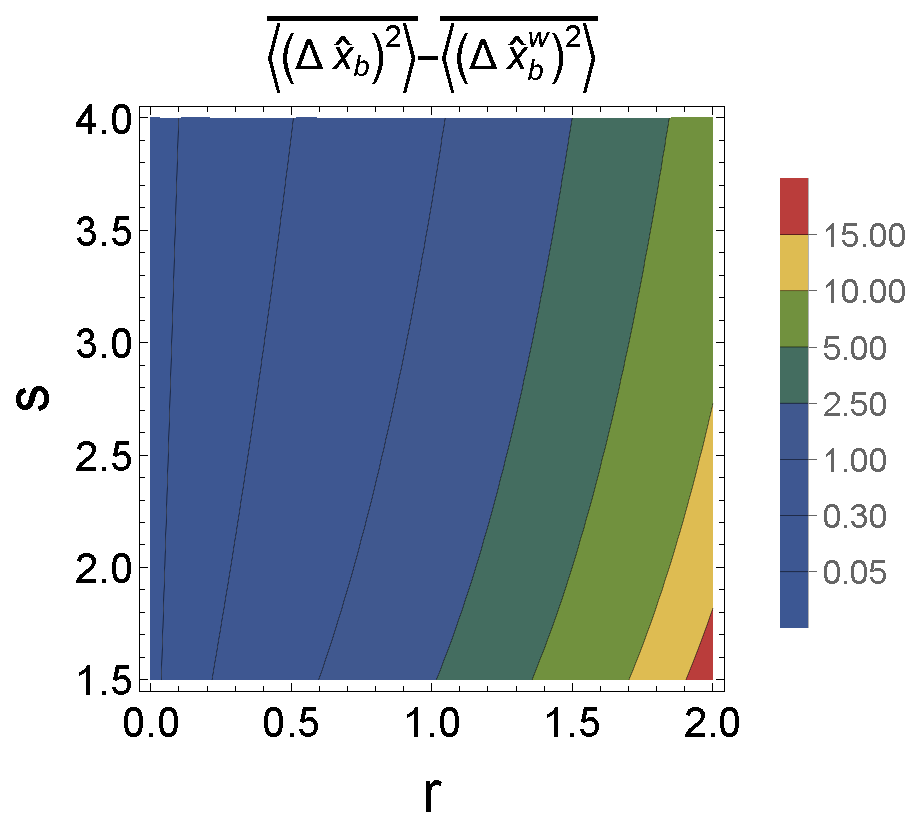
\includegraphics[width=.40\textwidth]{3Dsqz1_20190708.eps} {}
\end{center}
\caption{The difference between $\overline{\langle (\Delta \hat{x}_b)^2 \rangle}$ and $\overline{\langle (\Delta \hat{x}_b^{\rm{w}})^2 \rangle}$ as a function of $r$ and $s$ with single-mode squeezed states as input ($|\Psi^{\rm{in}}_1 \rangle = [\hat{D}(\alpha)\hat{S}(r)|0\rangle]^{\otimes K}$), with the number of input beams $K$, displacement operator $\hat{D}(\alpha) = e^{\alpha \hat{a}^{\dagger} - \alpha^{\ast} \hat{a}}$, and squeezing operator $\hat{S}(r) = e^{ (r /2)(\hat{a}^{\dagger 2} - \hat{a}^{2}) }$ (complex number $\alpha$ being the amplitude and real number $r$ the squeezing parameter). It shows that the difference is always larger than zero, namely the variance without WFS is greater than the one with WFS, which elucidates that WFS can reduce the averaged variance of the scattered modes. We have set the number of input beams $K=N$ ($N$ is the number of the transmission channels of the disordered medium).}
\label{3dsqz1}
\end{figure}


Note that the quadrature operators of a single-mode squeezed state can be written as
\begin{align}
\label{quadrature}
\hat{x}_{a'}^{\rm{in}} &= x + e^{-r} \hat{x}^{\rm{v}}_{a'},\\ \nonumber
\hat{p}_{a'}^{\rm{in}} &= p + e^{r} \hat{p}^{\rm{v}}_{a'},
\end{align}
where $x$ and $p$ [$\alpha = (x + i p)/2$] are the mean values of operators $\hat{x}_{a'}^{\rm{in}}$ and $\hat{p}_{a'}^{\rm{in}}$, respectively, and the operators $\hat{x}^{\rm{v}}_{a'}$ and $\hat{p}^{\rm{v}}_{a'}$ denote the  quadratures of the vacuum states. It is easy to find that $\langle \hat{x}_{a'}^{\rm{v}} \rangle =\langle \hat{p}_{a'}^{\rm{v}} \rangle = 0$,
$\langle \hat{x}_{a'}^{\rm{in}} \rangle = x$,
$\langle \hat{p}_{a'}^{\rm{in}} \rangle = p$.
Then
$\langle (\Delta \hat{x}_{a'}^{\rm{in}})^2 \rangle = \langle (\hat{x}_{a'}^{\rm{in}})^2 \rangle - \langle \hat{x}_{a'}^{\rm{in}} \rangle^2 = e^{-2r}$, $\langle (\Delta \hat{p}_{a'}^{\rm{in}})^2 \rangle = \langle (\hat{p}_{a'}^{\rm{in}})^2 \rangle - \langle \hat{p}_{a'}^{\rm{in}} \rangle^2 = e^{2r}$,
$\langle (\Delta \hat{x}_{b'}^{\rm{in}})^2 \rangle = \langle (\Delta \hat{p}_{b'}^{\rm{in}})^2 \rangle = 1$, $\langle \hat{x}_{a'}^{\rm{in}} \hat{x}_{a''}^{\rm{in}} \rangle - \langle \hat{x}_{a'}^{\rm{in}}\rangle \langle \hat{x}_{a''}^{\rm{in}} \rangle = 0$ ($a' \neq a''$), $\langle \hat{p}_{a'}^{\rm{in}} \hat{p}_{a''}^{\rm{in}} \rangle - \langle \hat{p}_{a'}^{\rm{in}}\rangle \langle \hat{p}_{a''}^{\rm{in}} \rangle = 0$ ($a' \neq a''$). Combining all these arguments and Eqs. (\ref{var20}), (\ref{var2a}), (\ref{var2b}), one can obtain
\begin{align}
\label{sqz1xb}
\langle(\Delta \hat{x}_b^{\rm{w}})^2 \rangle &= 1 - \sum_{a'}^{K}T_{a'b} (1 - e^{-2r}), \\ \nonumber
\langle(\Delta \hat{p}_b^{\rm{w}})^2 \rangle &= 1 + \sum_{a'}^{K}T_{a'b} ( e^{2r} - 1),
\end{align}
where we have used $\sum_{a'} T_{a'b} + \sum_{b'} R_{b'b} = 1$ (see Append. \ref{derivation} in detail).


\begin{figure}[htb]
\begin{center}
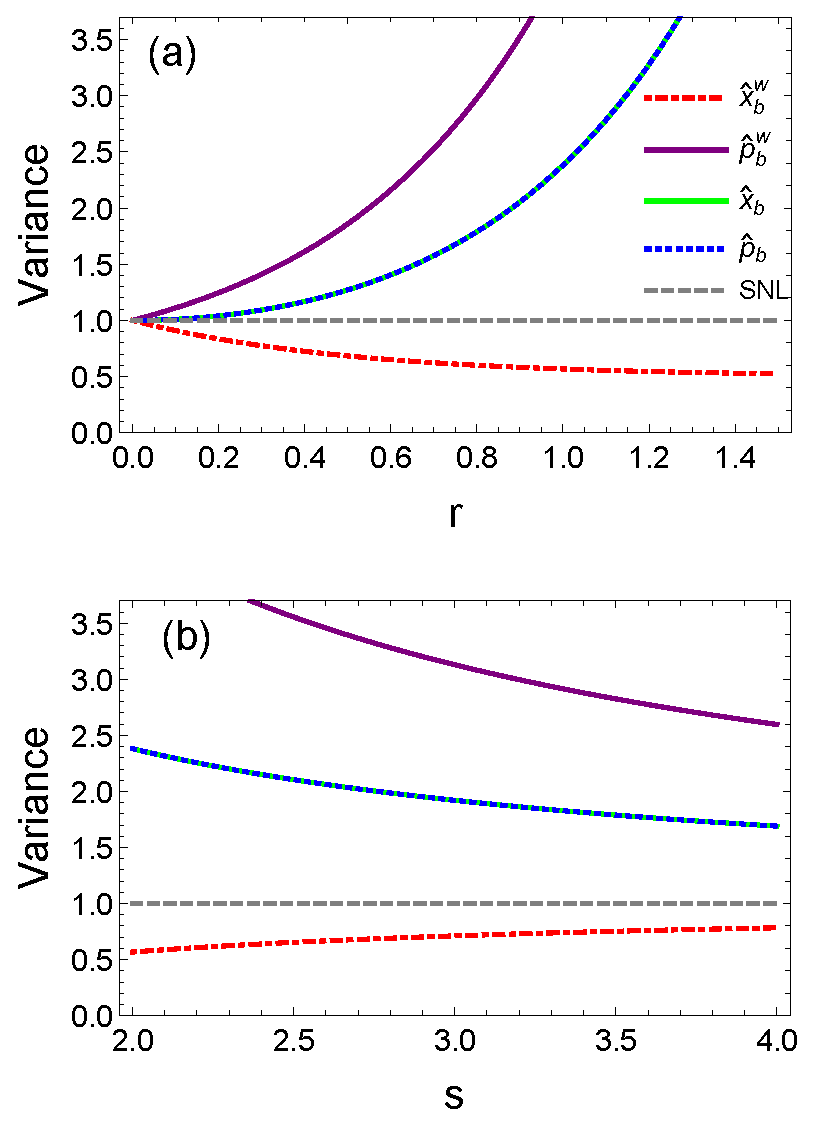
\includegraphics[width=.40\textwidth]{sqz1a20190830.eps} {}
\end{center}
\caption{The averaged variances $\overline{\langle (\Delta \hat{O})^2 \rangle}$ ($\hat{O} =$$\hat{x}_b^{\rm{w}}$, $\hat{p}_b^{\rm{w}}$, $\hat{x}_b$, $\hat{p}_b$) versus (a) $r$ and (b) $s$ with single-mode squeezed states as input, $| \Psi_1^{\rm{in}} \rangle = [\hat{D}(\alpha) \hat{S}(r) |0\rangle]^{\otimes K}$. The red-dash-dotted, purple-solid, green-solid, blue-dotted, and gray-dashed lines denote the cases of $\hat{x}_b^{\rm{w}}$, $\hat{p}_b^{\rm{w}}$, $\hat{x}_b$, $\hat{p}_b$, and SNL, respectively. It is worthy pointing out that since the averaged variances of $\hat{x}_b$ and $\hat{p}_b$ are equal to each other, the corresponding curves are completely coincident. Parameters used are: (a) $s = 2$ and (b) $r = 1$. We have set the number of input beams $K=N$ ($N$ denotes the number of the transmission channels of the disordered medium). }
\label{xr}
\end{figure}

By averaging over all ensembles of disorders, Eq. (\ref{sqz1xb}) is then reduced to
\begin{align}
\label{sqz1xbm}
\overline{\langle(\Delta \hat{x}_b^{\rm{w}})^2\rangle} &= 1 - K \overline{T_{a'b}} (1 - e^{-2r}) \\ \nonumber
&= 1 - \frac{K}{Ns} (1 - e^{-2r}), \\ \nonumber
\overline{\langle(\Delta \hat{p}_b^{\rm{w}})^2\rangle} &= 1 + \frac{K}{Ns}  (e^{2r} - 1),
\end{align}
where the overline indicates the average over all ensembles ($N$ means the number of transmission channels, $K$ the number of input beams, $s$ the disorder degree, and $r$ the squeezing parameter of the input states). It is worthy pointing out that the result [Eq. (12)] is only suitable for the variance averaged over many disorder realizations whereas the result [Eq. (11)] without disorder average only applies to a measurement performed on a particular disorder sample. When $r=0$, (i.e. coherent states as input), the averaged output noise via WFS, $\overline{\langle(\Delta \hat{x}_b^{\rm{w}})^2\rangle} = \overline{\langle(\Delta \hat{p}_b^{\rm{w}})^2\rangle} = 1$, is at the shot-noise level (SNL) which is defined as the quantum fluctuation of quadrature of the coherent state ($\langle(\Delta \hat{x}_{\rm{SNL}})^2\rangle = 1$). Actually, when coherent states are injected, the scattered modes are still coherent states due to the linear splitting process in a disordered medium. Hence, the output noise is naturally at the SNL. Nevertheless, when $r>0$ (i.e. squeezed states as input), it is found that the averaged output noise via WFS always reaches below the SNL ($\overline{\langle(\Delta x_b^{\rm{w}})^2\rangle}  < 1$).

For comparison, the averaged quantum fluctuation without WFS is also considered and is given by 
\begin{align}
\label{sqz1var2xxx}
\overline{\langle (\Delta \hat{x}_{b})^2 \rangle} = \overline{\langle (\Delta \hat{p}_{b})^2 \rangle} = 1+ \frac{K}{Ns} [\cosh (2r) - 1],
\end{align}
where the detailed derivation is shown in Append. \ref{appsinglemode}. When the number of input beams $K$ is reduced to one, one obtain $\overline{\langle (\Delta \hat{x}_{b})^2 \rangle} = \overline{\langle (\Delta \hat{p}_{b})^2 \rangle} = 1+ [\cosh (2r) - 1]/(Ns)$ which reproduces the result in Ref. \cite{lodahl2006b}. On the other hand, when $r=0$ (i.e. coherent-state input), Eq. (13) is reduced to $\overline{\langle (\Delta \hat{x}_{b})^2 \rangle} = \overline{\langle (\Delta \hat{p}_{b})^2 \rangle} = 1$ corresponding to the SNL. In other words, $r=0$ (i.e. without quantum effect) leads to the fact that the averaged quantum noise is always at the SNL regardless of what $s$ is. When $r>0$ (i.e. squeezed-state input), the averaged quantum noise is always above the SNL, which indicates that the scattered mode without WFS shows an averaged quantum noise above the SNL. In this sense, the quantum effect ($r> 0$) plays a dominate role in determining the averaged quantum noise. The difference between the averaged variances with WFS and without WFS is plotted in Fig. \ref{3dsqz1}. It is easily found that this difference is always positive, meaning that the averaged variance without WFS is greater than the one with WFS, which yields that the averaged quantum noise is suppressed via WFS. 

Fig. \ref{xr}(a) compares the averaged variances with and without WFS as a function of $r$. As shown in Fig. \ref{xr}(a), the red-dash-dotted, purple-solid, green-solid, blue-dotted, and gray-dashed lines denote the averaged variances of $\hat{x}_b^{\rm{w}}$, $\hat{p}_b^{\rm{w}}$, $\hat{x}_b$, $\hat{p}_b$, and SNL, respectively. It can be seen that the averaged variance ($\hat{x}_b$) without WFS is always above the SNL whereas the one ($\hat{x}_b^{\rm{w}}$) with WFS is below the SNL. In other words, the WFS can suppress the averaged quantum noise, even below the SNL. With the increase of $r$, the averaged variance without WFS decreases whereas the one with WFS increases. It is worthy noting that when WFS is performed, the averaged variance of $\hat{x}_b^{\rm{w}}$ reaches below the SNL whereas the averaged variance of $\hat{p}_b^{\rm{w}}$ is still above the SNL. Similarly, in Fig. \ref{xr}(b), the averaged variances of scattered modes versus $s$ are plotted. It is shown that as $s$ increases the averaged variance without WFS decreases. On the contrary, with the increase of $s$, the averaged variance with WFS increases. 


\subsection{Two-mode squeezed states as input}

\begin{figure}[htb]
\begin{center}
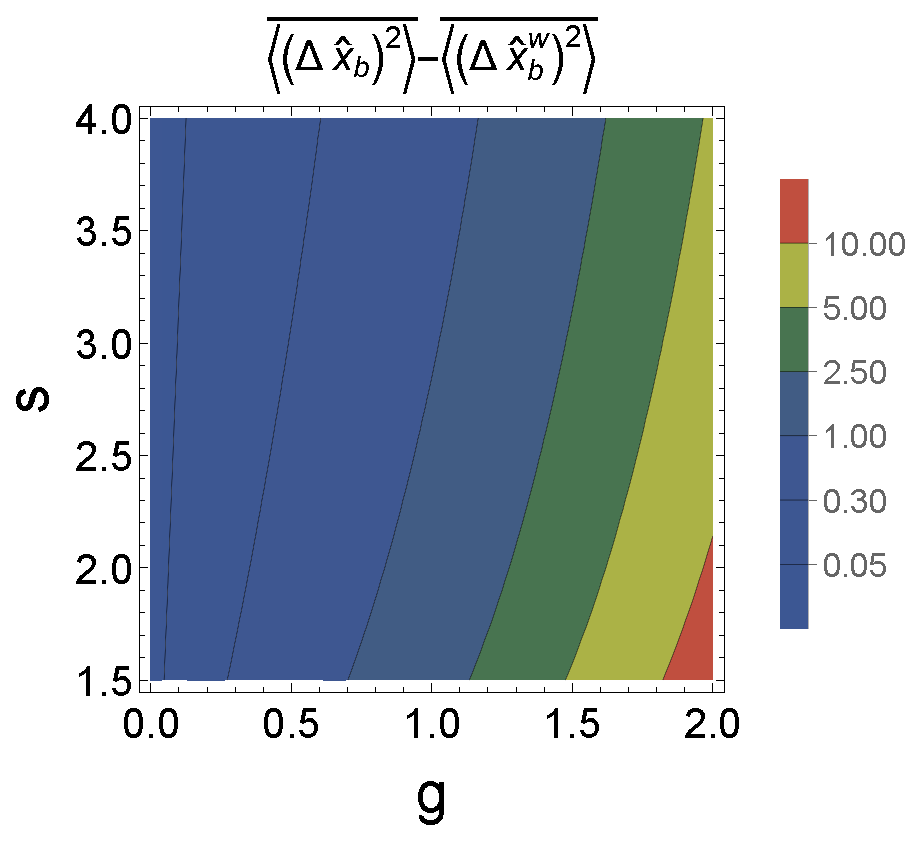
\includegraphics[width=.40\textwidth]{3Dsqz2_20190708.eps} {}
\end{center}
\caption{The difference between $\overline{\langle (\Delta \hat{x}_b)^2 \rangle}$ and $\overline{\langle (\Delta \hat{x}_b^{\rm{w}})^2 \rangle}$ as a function of $g$ and $s$ with two-mode squeezed states as input, $| \Psi_2^{\rm{in}} \rangle = \{\hat{D}_{A}(\alpha)  \hat{D}_{B}(\beta) \hat{S}_{AB}(\zeta) |0\rangle_A |0\rangle_B \}^{\otimes K/2}$ with displacement operators $\hat{D}_A(\alpha) = e^{\alpha \hat{a}_A^{\dagger} - \alpha^{\ast} \hat{a}_A}$, $\hat{D}_B(\beta) = e^{\beta \hat{a}_B^{\dagger} - \beta^{\ast} \hat{a}_B}$, two-mode squeezing operator $\hat{S}_{AB}(g) = e^{(-\zeta\hat{a}_{A}^{\dagger}\hat{a}_{B}^{\dagger} +\zeta^{\ast} \hat{a}_{A}\hat{a}_{B}) }$ ($\zeta = g e^{i \phi_{g}}$, real number $g$ denoting the squeezing parameter and real number $\phi_{g}$ the squeezing angle), and the number of input beams $K$. It shows that the difference is always greater than zero, which elucidates that the WFS can reduce the averaged variance of quadratures of scattered modes. We have set the number of input beams $K=N$ ($N$ is the number of transmission channels of the disordered medium).}
\label{3dsqz2}
\end{figure}

\begin{figure}[htb]
\begin{center}
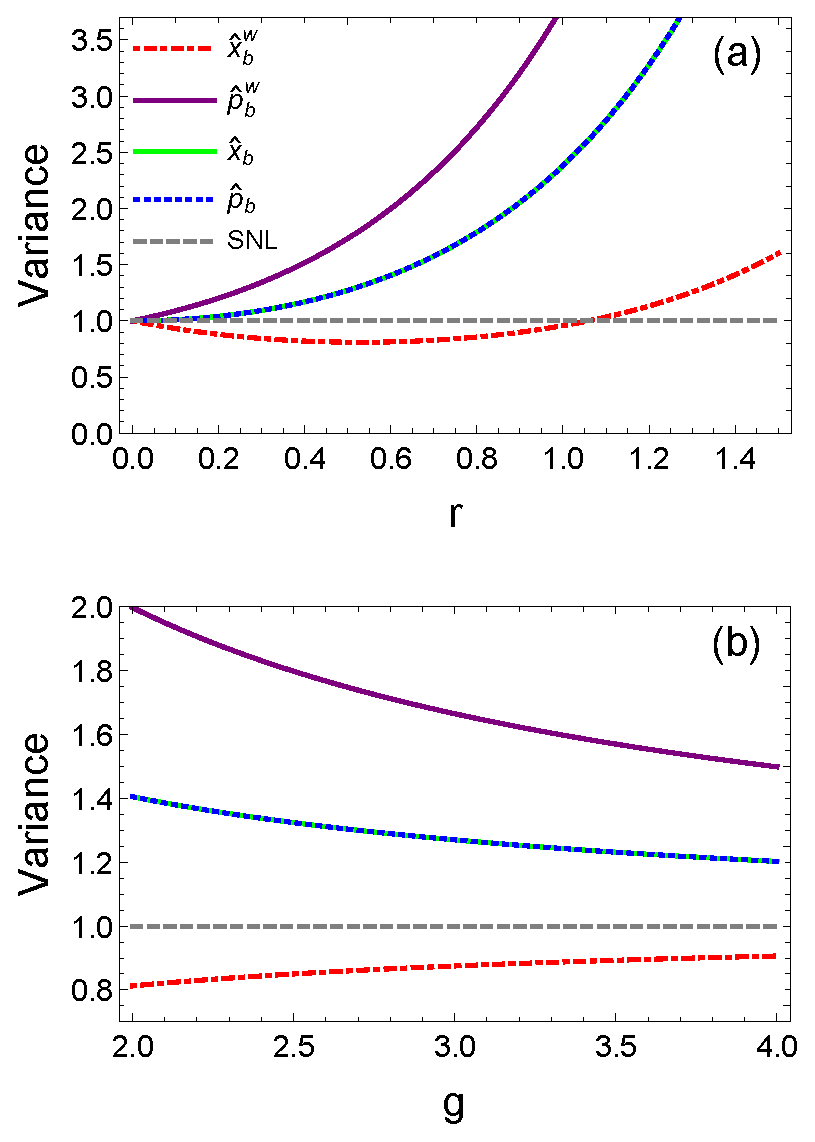
\includegraphics[width=.40\textwidth]{sqz2a20190830.eps} {}
\end{center}
\caption{The averaged variances $\overline{\langle (\Delta \hat{O})^2 \rangle}$ ($\hat{O} =$$\hat{x}_b^{\rm{w}}$, $\hat{p}_b^{\rm{w}}$, $\hat{x}_b$, $\hat{p}_b$) versus (a) $g$ and (b) $s$ with two-mode squeezed states as input, $| \Psi_2^{\rm{in}} \rangle = \{\hat{D}_{A}(\alpha) \hat{D}_{B}(\beta) \hat{S}_{AB}(\zeta) |0\rangle_A |0\rangle_B \}^{\otimes K/2}$. The red-dash-dotted, purple-solid, green-solid, blue-dotted, and gray-dashed lines denote the cases of $\hat{x}_b^{\rm{w}}$, $\hat{p}_b^{\rm{w}}$, $\hat{x}_b$, $\hat{p}_b$, and SNL, respectively. It is worthy pointing out that since the averaged variances of $\hat{x}_b$ and $\hat{p}_b$ are equal to each other, the corresponding curves are completely coincident. Parameters used are (a) $s = 2$, (b) $g = 0.6$. We have set the number of input beams $K=N$ ($N$ is the number of transmission channels of the disordered medium). }
\label{xr2}
\end{figure}


Since the two-mode squeezed state \cite{barnett2002} has a squeezed fluctuation similar to the single-mode squeezed state, we wonder whether the two-mode squeezed state  could also exhibit the quantum-noise reduction via WFS. 


Consider that the input is two-mode squeezed states, $| \Psi_2^{\rm{in}} \rangle = \{\hat{D}_{A}(\alpha) \hat{D}_{B}(\beta) \hat{S}_{AB}(\zeta) |0\rangle_A |0\rangle_B \}^{\otimes K/2}$ with number of the input modes $K$ ($K$ is even), displacement operators $\hat{D}_A(\alpha) = e^{\alpha \hat{a}_A^{\dagger} - \alpha^{\ast} \hat{a}_A}$, $\hat{D}_B(\beta) = e^{\beta \hat{a}_B^{\dagger} - \beta^{\ast} \hat{a}_B}$, and two-mode squeezing operator $\hat{S}_{AB}(\zeta) = e^{(-\zeta\hat{a}_{A}^{\dagger}\hat{a}_{B}^{\dagger} +\zeta^{\ast} \hat{a}_{A}\hat{a}_{B}) }$ ($\zeta = g e^{i \phi_{g}}$, the real number $g$ being the squeezing parameter and the real number $\phi_{g}$ denoting the squeezing angle).


For simplicity, let $\beta = \alpha$. Assume that $\alpha = (x + i p)/2$, and each pair of input modes $A = a'$ and $B = a'+K/2$ ($a' = 1,2,...,K/2$) constitutes a two-mode squeezed state. Then one can obtain $\langle \hat{x}_{a'}^{\rm{in}} \rangle = x$, $\langle \hat{p}_{a'}^{\rm{in}} \rangle = p$, $\langle \hat{x}_{b'}^{\rm{in}} \rangle = 0$, $\langle \hat{p}_{b'}^{\rm{in}} \rangle = 0$. And $\langle (\Delta \hat{x}_{a'}^{\rm{in}})^2 \rangle = 2 \sinh^2 g + 1$, $\langle (\Delta \hat{p}_{a'}^{\rm{in}})^2 \rangle = 2 \sinh^2 g + 1$,
$\langle (\Delta \hat{x}_{b'}^{\rm{in}})^2 \rangle = \langle (\Delta \hat{p}_{b'}^{\rm{in}})^2 \rangle = 1$. The covariance function between $\hat{x}_{a'}^{\rm{in}}$ and $\hat{x}_{a''}^{\rm{in}}$ can be described as
${\rm{cov}}(\hat{x}_{a'}^{\rm{in}}, \hat{x}_{a''}^{\rm{in}}) = \frac{1}{2}(\langle \hat{x}_{a'}^{\rm{in}} \hat{x}_{a''}^{\rm{in}} \rangle + \langle \hat{x}_{a''}^{\rm{in}} \hat{x}_{a'}^{\rm{in}} \rangle) - \langle \hat{x}_{a'}^{\rm{in}} \rangle \langle \hat{x}_{a''}^{\rm{in}} \rangle = \delta_{a',a''-K/2} 2 \cosh g \sinh g \cos \phi_g.$ It is worthy pointing out that these covariance functions vanish when the single-mode squeezed states are considered as inputs whereas they can not be ignored in the presence of two-mode squeezed input states. This is because there exists the nonclassical correlation between the two modes in each two-mode squeezed input state.


According to Eqs. (\ref{var20}), (\ref{var2a}), and (\ref{var2b}), the variances are found to be 
\begin{align}
\langle(\Delta \hat{x}_b^{\rm{w}})^2\rangle =& 1 + \sum_{a'}^{K}{T_{a'b} 2 \sinh^2 g}\\ \nonumber
&+\sum_{a'}^{K/2}{\sqrt{T_{a'b} T_{a'+K/2, b}} (4 \cos \phi_{g} \sinh g \cosh g )},
\end{align}
and
\begin{align}
\langle(\Delta \hat{p}_b^{\rm{w}})^2\rangle =& 1 + \sum_{a'}^{K}{T_{a'b} 2 \sinh^2 g}\\ \nonumber
&-\sum_{a'}^{K/2}{\sqrt{T_{a'b} T_{a'+K/2, b}} (4 \cos \phi_{g} \sinh g \cosh g )}.
\end{align}

To minimize variance $\langle(\Delta \hat{x}_b)^2\rangle$, one can set $\cos \phi_{g} = -1$ and obtain the minimum value
\begin{align}
\label{dx200a}
\langle(\Delta \hat{x}_b^{\rm{w}})^2\rangle =& 1 + \sum_{a'}^{K}{T_{a'b} 2 \sinh^2 g} \\ \nonumber
&- \sum_{a'}^{K/2}{\sqrt{T_{a'b} T_{a'+K/2, b}} (4  \sinh g \cosh g )}.
\end{align}
Meanwhile, $\langle(\Delta \hat{p}_b^{\rm{w}})^2\rangle$ is recast as
\begin{align}
\label{dp200a}
\langle(\Delta \hat{p}_b^{\rm{w}})^2\rangle =& 1 + \sum_{a'}^{K}{T_{a'b} 2 \sinh^2 g} \\ \nonumber
&+ \sum_{a'}^{K/2}{\sqrt{T_{a'b} T_{a'+K/2, b}} (4  \sinh g \cosh g )}.
\end{align}

By averaging over all disorder ensembles, the quantum fluctuations in Eqs. (\ref{dx200a}) and (\ref{dp200a}) are worked out as
\begin{align}
\label{sqz2var2}
\overline{\langle(\Delta \hat{x}_b^{\rm{w}})^2\rangle} &= 1 + 2K\overline{T_{a'b}} \sinh g ( \sinh g - \frac{\pi}{4} \cosh g)\\ \nonumber
& = 1 + \frac{2K}{Ns} \sinh g ( \sinh g - \frac{\pi}{4} \cosh g),
\end{align}
and
\begin{align}
\overline{\langle(\Delta \hat{p}_b^{\rm{w}})^2\rangle} &=  1 + \frac{2K}{Ns} \sinh g ( \sinh g + \frac{\pi}{4} \cosh g),
\end{align}
where $\overline{\sqrt{T_{a'b} T_{a'+K/2, b}}} = \overline{T_{a'b}} \pi/4$ is used and is proven in Append. \ref{rayleigh} for simplicity. Eq. (\ref{sqz2var2}) shows that if the modulated variance reaches below the SNL, it requires that $\sinh g - (\pi/4)\cosh g  < 0$, namely $ g < g_{\star} \equiv \rm{arctanh}$$( \pi / 4) \approx 1.06 $. That is to say, when $g < g_{\star}$, the averaged output quantum noise is below the SNL. However, when $g >g_{\star}$, it does not surpass the SNL. 


As a comparison, we also consider the mean variances in the absence of WFS
\begin{align}
\label{var3a}
\overline{\langle (\Delta \hat{x}_{b})^2 \rangle} &= 1+ 2 K \overline{T_{a'b}} \sinh^2 g \\ \nonumber
&= 1+ \frac{2 K}{Ns} \sinh^2 g, 
\end{align}
and
\begin{align}
\overline{\langle (\Delta \hat{p}_{b})^2 \rangle} &= 1+ \frac{2 K}{Ns} \sinh^2 g.
\end{align}
The corresponding deviation is shown in Append. \ref{apptwomode}. From Eq. (\ref{var3a}), it is noteworthy that the averaged output quantum noise without WFS is always above the SNL. Fig. \ref{3dsqz2} plots the difference between the averaged variances with and without WFS. It is shown that the difference is always greater than zero which indicates that WFS can reduce the averaged quantum fluctuation of the scattered mode.

In addition, Fig. \ref{xr2}(a) compares the averaged variances with and without WFS as a function of $g$. As shown in Fig. \ref{xr2}(a), the red-dash-dotted, purple-solid, green-solid, blue-dotted, and gray-dashed lines denote the averaged variances of $\hat{x}_b^{\rm{w}}$, $\hat{p}_b^{\rm{w}}$, $\hat{x}_b$, $\hat{p}_b$, and SNL, respectively. It is easy to verify that the averaged variance of $\hat{x}_b^{\rm{w}}$ with WFS is always smaller than the one without WFS. This yields that WFS can reduce the averaged output quantum noise. Different from the single-mode-squeezed-state input, the two-mode-squeezed-state one does not beat the SNL with WFS all the time. In fact, there exists a threshold $g_{\star} \approx 1.06$ which determines whether the reduced mean quantum noise reach below the SNL. When $g < g_{\star}$, the averaged variance with WFS can surpass the SNL whereas when $g > g_{\star}$, the one with WFS can not beat the SNL. In Fig. \ref{xr2}(b), the averaged variances with and without WFS are plotted as a function of $s$. Similar to the case of single-mode squeezed states, with $s$ increasing, the averaged variance in the absence of WFS decreases whereas the one in the presence of WFS increases as $s$ increases. 


\section{Discussion}

One may wonder why WFS can modulate the averaged quadrature fluctuations of the scattered light of a disordered medium. Here we will provide an intuitive interpretation of the quantum-noise reduction. Before any further explanation, let us turn attention to a simple case of the conventional balanced beam splitter (BS) which is a two-port device. For simplicity, we will take the single-mode-squeezed-state input as an example.

\subsection{Comparison with the two-port beam splitter}


\begin{figure}[htbp]
\begin{center}
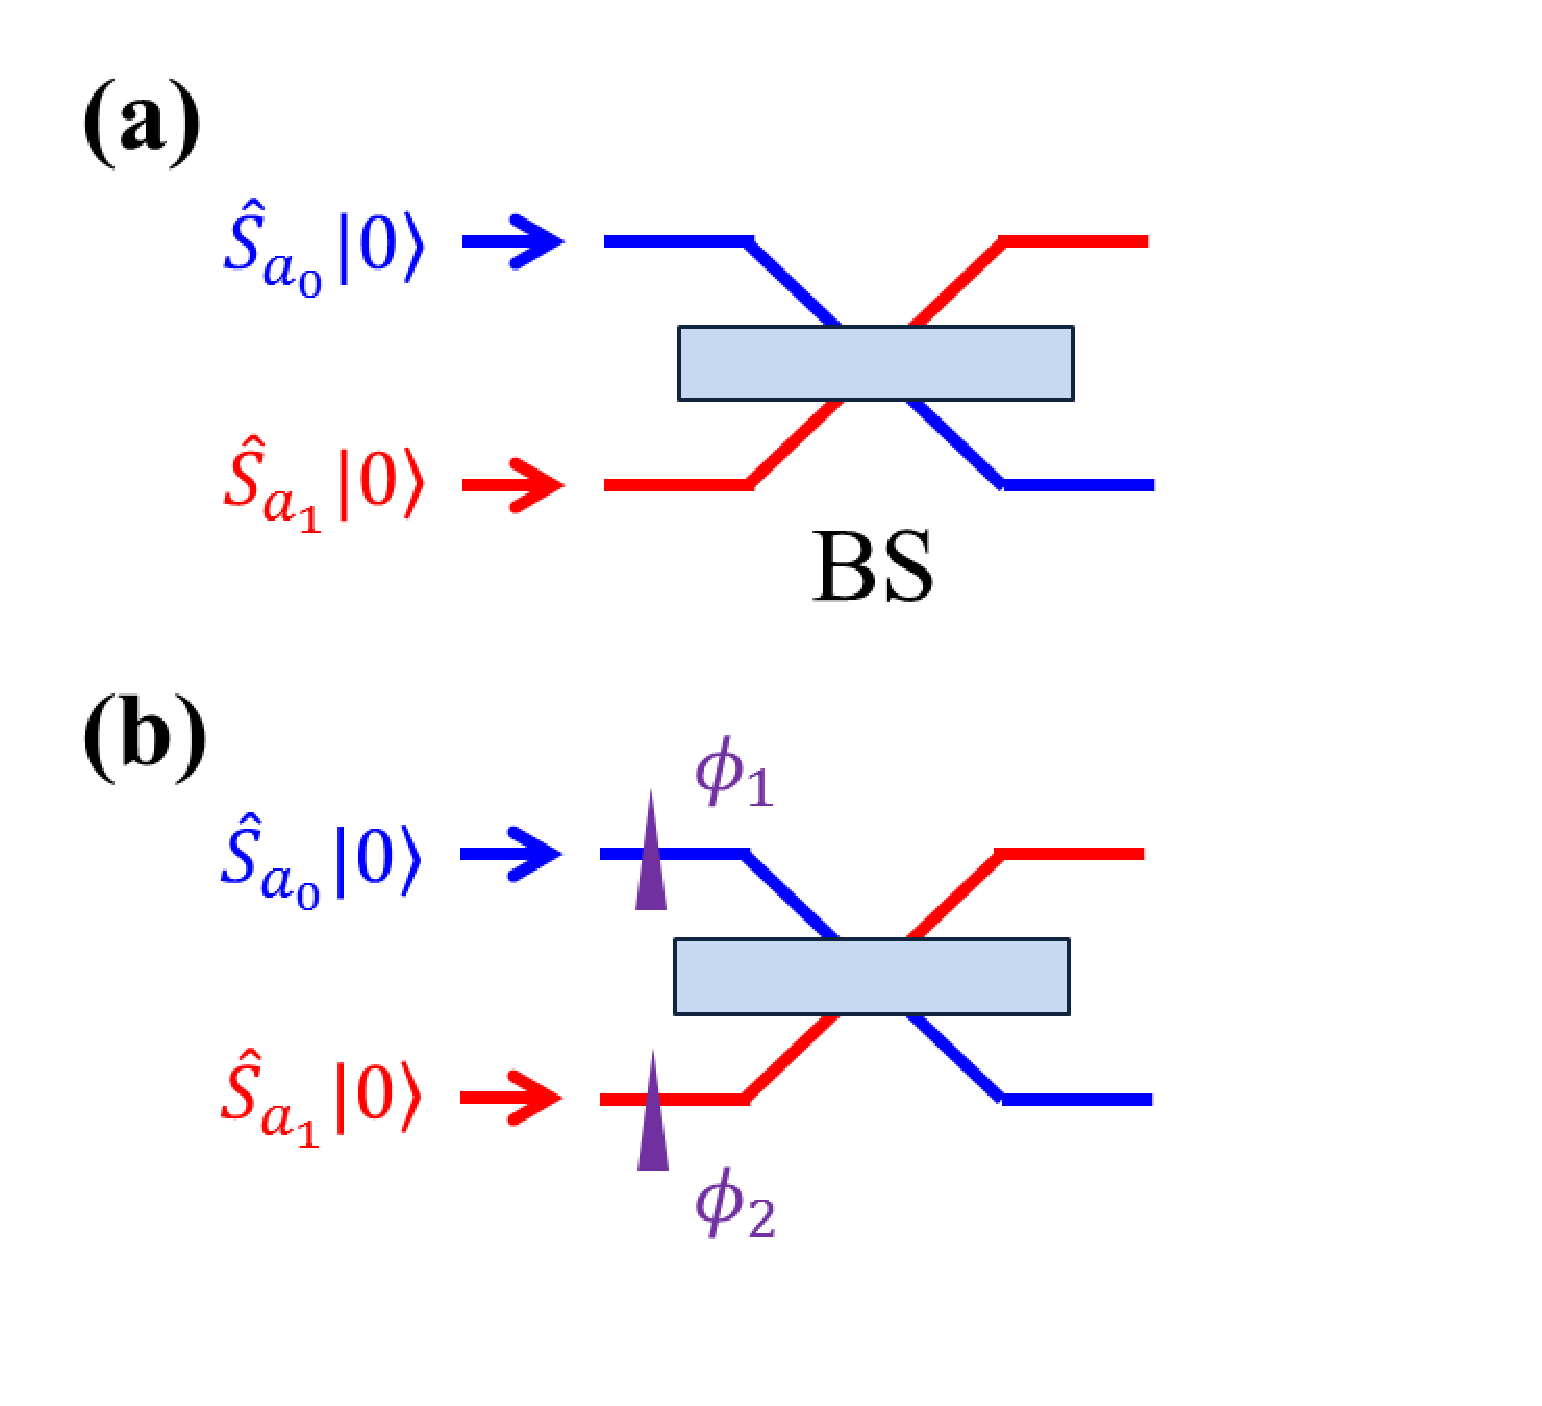
\includegraphics[width=.4\textwidth]{02_20190613_BS.eps} {}
\end{center}
\caption{Squeezed vacuum states propagating through a beam splitter (a) in the absence of WFS, and (b) in the presence of WFS. With a two-port beam splitter (BS), the WFS is equivalent to two phase shifters ($\phi_1$ and $\phi_2$) as depicted in (b).}
\label{bs12}
\end{figure}


For the BS, akin to the disordered medium, we consider the situation where the input is the single-mode squeezed vacuum states,
\begin{align}
|\Psi^{\rm{in}}_3\rangle = \hat{S}_{a_0}(r)|0\rangle \otimes \hat{S}_{a_1}(r)|0\rangle,
\end{align}
where $\hat{S}_{a_0}(r) = e^{(r/2) [(\hat{a}_0^{\rm{in}\dagger})^{ 2}-  (\hat{a}_0^{\rm{in} })^2]}$ ($\hat{S}_{a_1}(r) = e^{(r/2) [(\hat{a}_1^{\rm{in}\dagger})^{ 2}-  (\hat{a}_1^{\rm{in} })^2]}$) is the single-mode squeezing operator with $\hat{a}_0^{\rm{in} \dagger}$ ($\hat{a}_1^{\rm{in} \dagger}$) and $\hat{a}_0^{\rm{in}}$ ($\hat{a}_1^{\rm{in}}$) indicating the creation and annihilation operators of the input mode $0$ ($1$) and $r$ denoting the squeezing parameter. Two circumstances will be compared: (I) in the absence of WFS and (II) in the presence of WFS as illustrated in Figs. \ref{bs12}(a) and \ref{bs12}(b), respectively.

In the case I [Fig. \ref{bs12}(a)], without WFS, after passing through BS, the output state can be written as
\begin{align}
\label{outbswithoutWFS}
|\Psi^{\rm{out}}_3\rangle &= e^{i r [\hat{a}_0^{\rm{out}\dagger} \hat{a}_1^{\rm{out}\dagger} +  \hat{a}_0^{\rm{out} } \hat{a}_1^{\rm{out} }]}|0\rangle \otimes |0\rangle,
\end{align}
where $\hat{a}_0^{\rm{out} \dagger}$ ($\hat{a}_1^{\rm{out} \dagger}$) and $\hat{a}_0^{\rm{out}}$ ($\hat{a}_1^{\rm{out}}$) mean the creation and annihilation operators of the output mode $0$ ($1$). For clarity, the calculation is shown in Append. \ref{bsabsence}. As a matter of fact, the output in Eq. (\ref{outbswithoutWFS}) is the so-called two-mode squeezed vacuum state \cite{barnett2002}. After tracing over the output mode $1$, the reduced state of the output denotes the mode $0$ which is a thermal state. The corresponding variance of output mode $0$ can be worked out as
\begin{align}
\label{plus2r}
\langle (\Delta \hat{x}_{0}^{\rm{out}})^2 \rangle = 2 \sinh^2 r + 1 ,
\end{align} 
where $\hat{x}_{0}^{\rm{out}} \equiv \hat{a}_{0}^{\rm{out} \dagger} + \hat{a}_{0}^{\rm{out}}$. It is easy to check that when $r>0$, the output quantum noise of mode $0$ is always above the SNL which is similar to the case of single-mode squeezed input states in the disordered medium without WFS. 

\begin{figure*}[htb]
\begin{center}
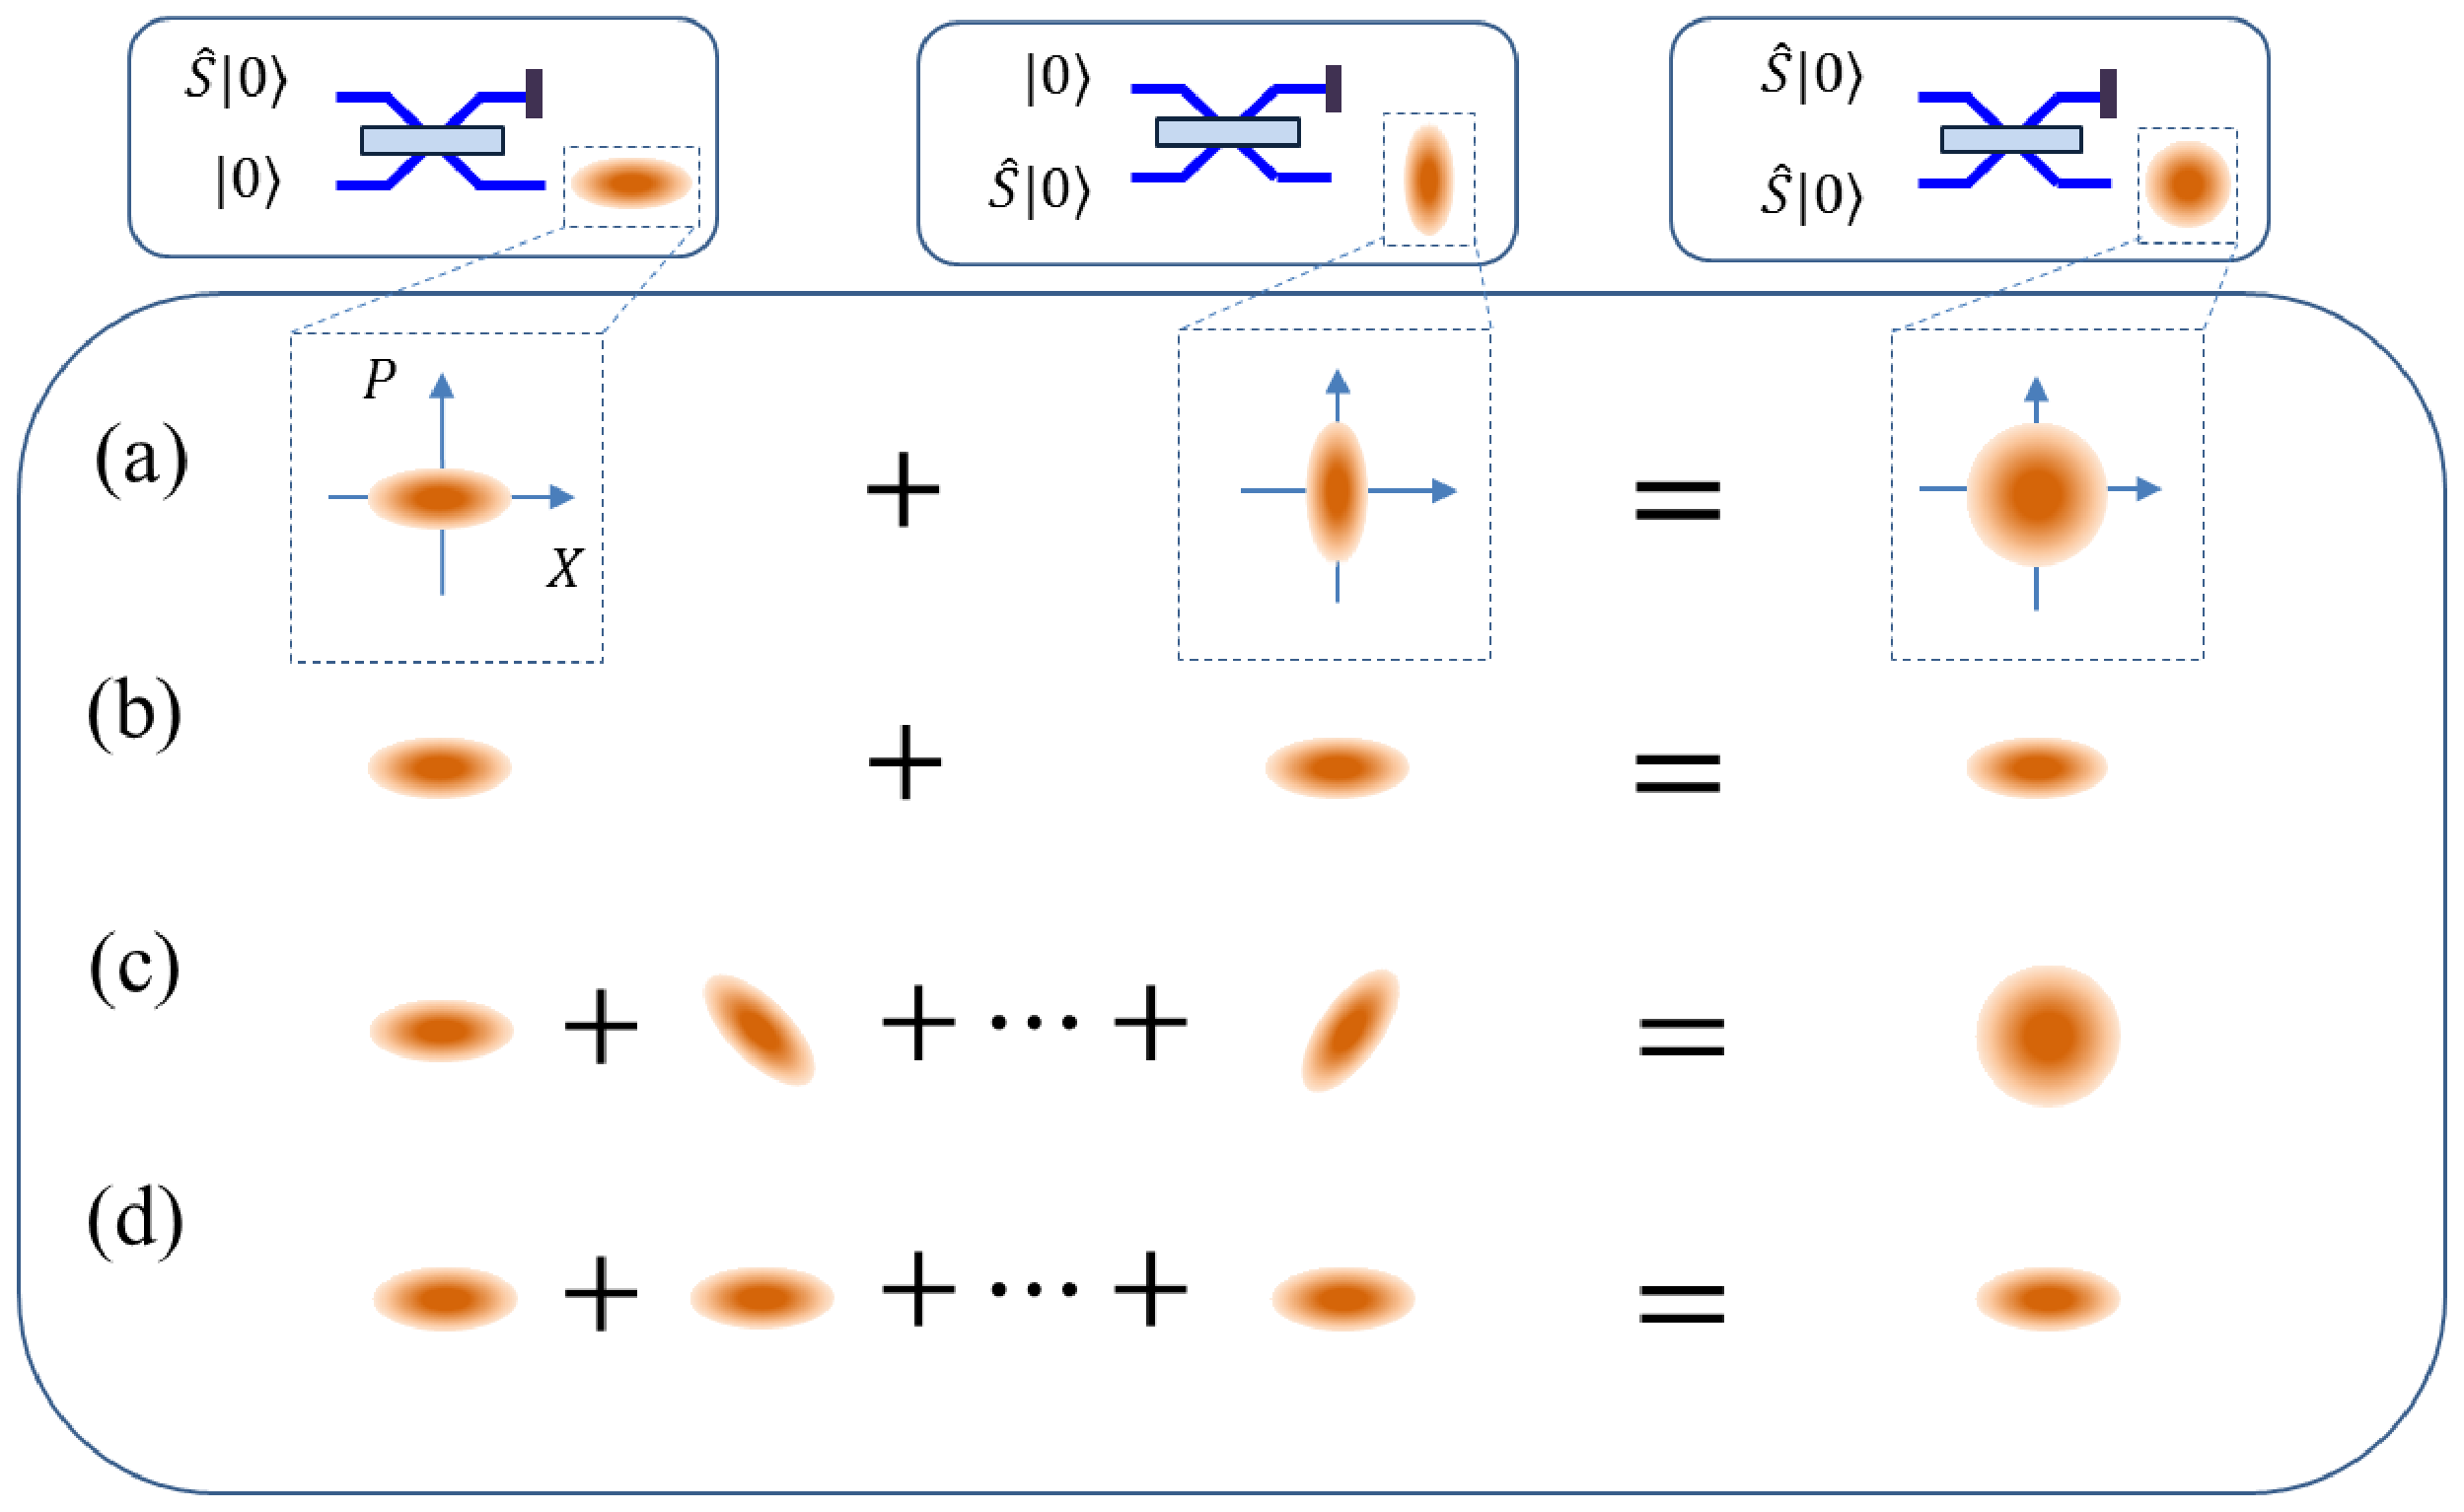
\includegraphics[width=.75\textwidth]{01_20190612_illustration.eps} {}
\end{center}
\caption{Qualitative description of the output states in phase space. The output states correspond to (a) without and (b) with WFS in a two-port beam splitter, (c) without and (d) with WFS in a multiple-port disordered medium. Note that each state of the left-hand side of the "equality" represents the output light which corresponds to each individual input beam as input separately. The term of the right-hand side denotes the final output state which is related to the case of all the initial light as input simultaneously. When mixing two output squeezed states (a) with different squeezing angles, the final output state would not achieve the optimal minimum variance, and (b) with the same squeezing angle, the final output state would achieve the optimal minimum variance. If mixing multiple squeezed states (c) with random squeezing angles, the final state would have a quantum fluctuation above the SNL, and (d) with the same squeezing angle, the final state would achieve the optimal minimum variance. It is obvious that rotating all squeezing angles in the same direction is a valid method of suppressing the final quantum noise. Actually, this reduction occurs as a result of destructive interference of quantum noise. Since WFS plays an essential role in manipulating the direction of squeezing angle, it can modulate the final quantum fluctuation. }
\label{illustration}
\end{figure*}

Consider the case II where the WFS is performed as depicted in Fig. \ref{bs12}(b). The WFS is actually equivalent to two phase shifters acting on two input modes. Without loss of generality, we may consider the two phase shifters to be $\phi_1$ and $\phi_2$, respectively. 

After $|\Psi^{\rm{in}}_3 \rangle$ propagates through the BS, the output state can be written as
\begin{align}
\label{eq22}
|\Psi^{\rm{out,w}}_3\rangle = e^{(r/2) [(\hat{a}_0^{\rm{out} })^2 - (\hat{a}_0^{\rm{out}\dagger})^{ 2}] - (r/2) [(\hat{a}_1^{\rm{out} })^2 - (\hat{a}_1^{\rm{out}\dagger})^{ 2}]}|0\rangle \otimes |0\rangle,
\end{align}
where we have set $\phi_1 = \pi/2$ and $\phi_2 = 0$ (see Append. \ref{bspresence}). From Eq. (\ref{eq22}), it is found that each output mode is a single-mode squeezed state. Then the variance of quadrature of output mode $0$ is calculated out to
\begin{align}
\label{minus2r}
\langle (\Delta \hat{x}_{0}^{\rm{out,w}})^2 \rangle = e^{-2r},
\end{align} 
where the output noise is below the SNL. This is similar to the single-mode squeezed states in the disordered medium with WFS.

Comparing Eqs. (\ref{plus2r}) and (\ref{minus2r}), one can easily see that the output noise with WFS is smaller than the one without WFS. This indicates that the WFS can reduce the variance of output quadrature, which is due to the destructive interference of quantum noise \cite{elste2009}. A detailed explanation will be presented in next subsection.

\subsection{Quantum-noise reduction resulting from uniform squeezing angles via WFS}

To illustrate quantum-noise reduction intuitively, we plot the output states in phase space in Fig. \ref{illustration}. Fig. \ref{illustration}(a) corresponds to the case I of a BS without WFS, the state of the left-hand side of the "equality" denotes the output beam which results from each single beam as input separately while the state on the right-hand side indicates the final output state with both beams as input simultaneously. Without WFS, the output states of the left-hand side present different squeezing angles. As a consequence, the final output state is the thermal state which shows a quantum fluctuation above the SNL. 

With the help of WFS in a BS, as depicted in Fig. \ref{illustration}(b), the output states of the left-hand side of the "equality" demonstrate in an uniform squeezing angle. As a result, the final output maintains a sub-shot noise. In other words, this final state has a quantum fluctuation below the SNL. We call this phenomenon the destructive interference of quantum noise.

By contrast, Figs. \ref{illustration}(c) and \ref{illustration}(d) are related to the disordered medium, a multiple-port optical device, without and with WFS. Similarly, in the absence of WFS [Fig. \ref{illustration}(c)], the output states of the left-hand side have randomly distributed squeezing angles. This leads to the final output state with a quantum fluctuation which is larger than the SNL. However, in the presence of WFS [Fig. \ref{illustration}(d)], squeezing angles are distributed uniformly. As a consequence, the final output state has a squeezed quantum fluctuation below the SNL.

From Fig. \ref{illustration}, it is evident that WFS modulates the quantum fluctuation via rotating the squeezing angles. Without WFS, the output squeezing angles are randomly distributed which gives rise to a final output quantum fluctuation above the SNL. In the presence of WFS, it rotates the squeezing angles in the same direction which makes the final output quantum fluctuation below the SNL owing to the destructive interference of quantum noise.

\section{Conclusion}
In summary, the effect of wavefront shaping on the averaged quantum fluctuations of quadratures of scattered modes is investigated. It is clarified that wavefront shaping leads to reduction of averaged quantum noise of scattered beams. Particularly, when the input is the single-mode squeezed states, the averaged quantum fluctuation can always be decreased below the shot-noise level. If the two-mode squeezed states are considered as input, the averaged quantum fluctuation can be suppressed, but it is not always below the shot-noise level. As a matter of fact, there exits a threshold $g_{\star}$ which determines whether the reduced mean quantum noise reaches below the shot-noise level. When the input squeezing parameter is smaller than the threshold $g < g_{\star} \approx 1.06$, the reduced mean quantum noise can always achieve below the SNL whereas the one is always above the shot-noise level when $g > g_{\star} \approx 1.06$. Moreover, with the increasing of disorder strength, the degree of reduction of the averaged quantum noise decreases. Above all, the reduction of averaged quantum noise results from destructive interference of quantum noise via wavefront shaping. 

These results may have applications in quantum information processing, for instance, sub-wavelength imaging \cite{putten2011,park2014,jang2018,chen2018}, where the disordered medium plays a role in focusing light as a scattering superlens. Recall that our proposal with squeezed-state sources provides the output with a sub-shot noise, which may improve the resolution in imaging by boosting the signal-to-noise ratio.


\section{Acknowledge}
We thank Prof. Song Sun for his insightful suggestions. This work was supported by the Science Challenge Program (Grant No. TZ2018003-3) and National Natural Science Foundation of China (Grant Nos. 61875178 and 11605166).




%%%%%%%%%%%%%%%%%%%%%%%%%%%%%%%%%%%%%%%
%\bibliography{loss0928}
%%%%%%%%%%%%%%%%%%%%%%%%%%%%%%%%%%%%%%%
\begin{thebibliography}{99}
\newcommand{\enquote}[1]{``#1''}

\bibitem{b1998} C. W. J. Beenakker, \enquote{Thermal radiation and amplified spontaneous emission from a random medium,} Phys. Rev. Lett. \textbf{81}, 1829 (1998). 

\bibitem{smolka2009} S. Smolka, A. Huck, U. L. Anderson, A. Lagendijk, and P. Lodahl, \enquote{Observation of spatial quantum correlations induced by multiple scattering of nonclassical light,} Phys. Rev. Lett. \textbf{102}, 193901 (2009).

\bibitem{peeters2010} W. H. Peeters, J. J. D. Moerman, and M. P. van Exter, \enquote{Observation of two-photon speckle patterns,} Phys. Rev. Lett. \textbf{104}, 173601 (2010).


\bibitem{Beenakker2000} C. W. J. Beenakker and M. Patra, \enquote{Photon shot noise,} Mod. Phys. Lett. B \textbf{13}, 337 (1999). 

\bibitem{patra1999} M. Patra and C. W. J. Beenakker, \enquote{Excess noise for coherent radiation propagating through amplifying random media,} Phys. Rev. A \textbf{60}, 4059 (1999).

\bibitem{patra2000} M. Patra, C. W. J. Beenakker, \enquote{Propagation of squeezed radiation through amplifying or absorbing random media,} Phys. Rev. A \textbf{61}, 063805 (2000). 

\bibitem{two2002} J. Tworzydlo and C. W. J. Beenakker, \enquote{Quantum optical communication rates through an amplifying random medium,} Phys. Rev. Lett. \textbf{89}, 043902 (2002).

\bibitem{lodahl2005a} P. Lodahl and A. Lagendijk, \enquote{Transport of quantum noise through random media,} Phys. Rev. Lett. \textbf{94}, 153905 (2005).
\bibitem{lodahl2005b} P. Lodahl, A. P. Mosk, and A. Lagendijk, \enquote{Spatial quantum correlations in multiple scattered light,} Phys. Rev. Lett. \textbf{95}, 173901 (2005).

\bibitem{gilead2015} Y. Gilead, M. Verbin, and Y. Silberberg, \enquote{Ensemble-averaged quantum correlation between path-entangled photons undergoing Anderson localization,} Phys. Rev. Lett. \textbf{115}, 133602 (2015).

\bibitem{wiersma2013} D. S. Wiersma, \enquote{Disordered photonics,} Nat. Photon. \textbf{7}, 188 (2013).

\bibitem{vellekoop2010np} I. M. Vellekoop, A. Lagendijk, and A. P. Mosk, \enquote{Exploiting disorder for perfect focusing,} Nat. Photon. \textbf{4}, 320 (2010).

\bibitem{lahini2010} Y. Lahini, Y. Bromberg, D. N. Christodoulides, and Y. Siberberg, \enquote{Quantum correlations in two-particle Anderson localization,} Phys. Rev. Lett. \textbf{105}, 163905 (2010).

\bibitem{defienne2016} H. Defienne, M. Barbieri, I. A. Walmsley, B. J. Smith, and S. Gigan, \enquote{Two-photon quantum walk in a multimode fiber,} Science Advances \textbf{2}, e1501054 (2016).


\bibitem{rotter2017} S. Rotter and S. Gigan, \enquote{Light fields in complex media: mesoscopic scattering meets wave control,} Rev. Mod. Phys. \textbf{89}, 015005 (2017).

\bibitem{leonetti2013} M. Lenonetti, C. Conti, and C. Lopez, \enquote{Switching and amplification in disordered lasing resonators,} Nat. Commun. \textbf{4}, 1740 (2013).

\bibitem{starshynov2016} I. Starshynov, J. Bertolotti, and J. Anders, \enquote{Quantum correlation of light scattered by disordered media,} Opt. Expr. \textbf{5}, 4662 (2016).

\bibitem{an2018} C. Ma, Y. S. Wang, and J.-H. An, \enquote{Floquet engineering of localized propagation of light in a waveguide array,} Phys. Rev. A \textbf{97}, 023808 (2018).

\bibitem{walschaers2016} M. Walschaers, F. Schlawin, T. Wellens, and A. Buchleitner, \enquote{Quantum transport on disordered and noisy networks: an interplay of structural complexity and uncertainty,} Annual Review of Condensed Matter Physics \textbf{7}, 223 (2016).

\bibitem{xu2017a} Y. Xu, H. Zhang, Y. Lin, and H. Zhu, \enquote{Light transport behaviours in quasi-1D disordered waveguides composed of random photonic lattices,} J. Mod. Opt. \textbf{64}, 1215 (2017).

\bibitem{xu2017b} Y. Xu, H. Zhang, Y. Lin, and H. Zhu, \enquote{Light transmission properties in inhomogeneously-disordered random
media,} Annalen der Physik \textbf{529} 1600225 (2017).

\bibitem{zhang2018} Z. Zhang, B. Zhang, Q. Feng, H. He, and Y. Ding, \enquote{Rapid measurement of transmission matrix with the sequential semi-definite programming method,} Chin. Phys. B \textbf{27}, 84201 (2018).

\bibitem{hong2017} P. Hong and G. Zhang, \enquote{Heisenberg-resolution imaging through a phase-controlled screen,} Optics Expr. \textbf{25}, 22789 (2017).

\bibitem{hong2018} P. Hong, \enquote{Two-photon imaging assisted by a dynamic random medium,} Appl. Phys. Lett. \textbf{113}, 101109 (2018).


\bibitem{wolterink2016} T. A. W. Wolterink, R. Uppu, G. Ctistis, W. L. Vos, K.-J. Boller, and P. W. H. Pinkse, \enquote{Programmable two-photon quantum interference in $10^3$ channels in opaque scattering media,} Phys. Rev. A \textbf{93}, 053817 (2016).

\bibitem{huisman2014} T. J. Huisman, S. R. Huisman, A. P. Mosk, and P. W. H. Pinkse, \enquote{Controlling single-photon Fock-state propagation through opaque scattering media,} Appl. Phys. B \textbf{116}, 603 (2014).

\bibitem{defienne2014} H. Defienne, M. Barbieri, B. Chalopin, B. Chatel, I. A. Walmsley, B. J. Smith, and S. Gigan, \enquote{Nonclassical light manipulation in a multiple-scattering medium,} Opt. Lett. \textbf{39}, 6090 (2014).

\bibitem{b2017} B. $\breve{\text{S}}$kori\'{c}, P. W. H. Pinkse, and A. P. Mosk, \enquote{Authenticated communication from quantum readout of PUFs,} Quantum Inf. Processing \textbf{16}, 200 (2017).


\bibitem{goorden2014} S. A. Goorden, M. Horstmann, A. P. Mosk, B. $\breve{\text{S}}$kori\'c, and P. W. H. Pinkse, \enquote{Quantum-secure authentication of a physical unclonable key,} Optica \textbf{1}, 421 (2014).

\bibitem{nikolopoulos2017} G. M. Nikolopoulos and E. Diamanti, \enquote{Continuous-variable quantum authentication of physical unclonable keys,} Sci. Rep. \textbf{7}, 46047 (2017).

\bibitem{yao2016} Y. Yao, M. Gao, M. Li, and J. Zhang, \enquote{Quantum cloning attacks against PUF-based quantum authentication systems,} Quantum Inf. Processing \textbf{15}, 3311 (2016).

\bibitem{li2017} Q. Li, F. Chen, M. Li, H. Long, P. Sun, P. Wang, Y. Yao, and J. Zhang, \enquote{Simulation of physically unclonable function based on disordered photonic structure,} Optical and Quantum Electronics \textbf{49}, 122 (2017).

\bibitem{walls1983} D. F. Walls, \enquote{Squeezed states of light,} Nature \textbf{306}, 141 (1983).

\bibitem{lvovsky2015} A. I. Lvovsky, \enquote{Squeezed light,} Photonics: Scientific Foundations, Technology and Applications \textbf{1}, 121 (2015).


\bibitem{walls2007} D. F. Walls and G. J. Milburn, \enquote{Quantum optics,} (Springer Science \& Business Media, Berlin, 2007).

\bibitem{barnett2002} S. M. Barnett and P. M. Radmore, \enquote{Methods in theoretical quantum optics,} (Oxford University Press, 2002).

\bibitem{caves81}
C.~M. Caves, \enquote{Quantum-mechanical noise in an interferometer,} Phys.
  Rev. D \textbf{23}, 1693 (1981).

\bibitem{yurke86}
B.~Yurke, S.~L. McCall, and J.~R. Klauder, \enquote{SU(2) and SU(1,1) interferometers,} Phys. Rev. A \textbf{33}, 4033 (1986).

\bibitem{xiao1987precision}
M.~Xiao, L.-A. Wu, and H.~J. Kimble, \enquote{Precision measurement beyond the shot-noise limit,} Phys. Rev. Lett. \textbf{59}, 278 (1987).


\bibitem{beskrovnyy2005} V. N. Beskrovnyy and M. I. Kolobov, \enquote{Quantum limits of super-resolution in reconstruction of optical objects,} Phys. Rev. A \textbf{71}, 043802 (2005).

\bibitem{sokolov2004} I. V. Sokolov and M. I. Kolobov, \enquote{Squeezed-light sources for superresolving microscopy,} Opt. Lett. \textbf{29}, 703 (2004).


\bibitem{aasi2013} LIGO Scientific Collaboration, \enquote{Enhanced sensitivity of the LIGO gravitational wave detector by using squeezed states of light,} Nat. Photon. \textbf{7}, 613 (2013).

\bibitem{barsotti2018} L. Barsotti, J. Harms, and R. Schnabel, \enquote{Squeezed vacuum states of light for gravitational wave detectors,} Reports on Progress in Physics \textbf{82}, 016905 (2018).

\bibitem{mehmet2018} M. Mehmet and H. Vahlbruch, \enquote{High-efficiency squeezed light generation for gravitational wave detectors,} Classical and Quantum Gravity \textbf{36}, 015014 (2018).


\bibitem{ott2010} J. R. Ott, N. A. Mortensen, and P. Lodahl, \enquote{Quantum interference and entanglement induced by multiple scattering of light,} Phys. Rev. Lett. \textbf{105}, 090501 (2010).

\bibitem{li2019} D. Li, Y. Yao, and M. Li, \enquote{Statistical distribution of quantum correlation induced by multiple scattering
in the disordered medium,} Opt. Comm. \textbf{446}, 106 (2019).

\bibitem{lodahl2006b} P. Lodahl, \enquote{Quantum correlations induced by multiple scattering of quadrature squeezed light,} Opt. Expr. \textbf{14}, 6919 (2006).

\bibitem{vellekoop2007} I. M. Vellekoop and A. P. Mosk, \enquote{Focusing coherent light through opaque strongly scattering media,} Opt. Lett. \textbf{32}, 2309 (2007).

\bibitem{vellekoop2008} I. M. Vellekoop and A. P. Mosk, \enquote{Phase control algorithms for focusing light through turbid media,} Opt. Commun. \textbf{281}, 2071 (2008).

\bibitem{popoff2010} S. Popoff, G. Lerosey, M. Fink, A. C. Boccara, and S. Gigan, \enquote{Image transmission through an opaque material,} Nat. Commun. \textbf{1}, 81 (2010).



\bibitem{mosk2012} A. P. Mosk, A. Lagendijk, G. Lerosey, and M. Fink, \enquote{Controlling waves in space and time for imaging and focusing in complex media,} Nat. Photon. \textbf{6}, 283 (2012).


\bibitem{prl2019} D. Pierangeli, G. Marcucci, and C. Conti, \enquote{Large-scale photonic Ising machine by spatial light modulation,} Phys. Rev. Lett. \textbf{112}, 213902 (2019).


\bibitem{lum2016} D. J. Lum, J. C. Howell, M. S. Allman, T. Gerrits, V. B. Verma, S. W. Nam, C. Lupo, and S. Lloyd, \enquote{Quantum enigma machine: experimentally demonstrating quantum data locking,} Phys. Rev. A \textbf{94}, 022315 (2016).

\bibitem{putten2011} E. G. van Putten, D. Akbulut, J. Bertolotti, W. L. Vos, A. Lagendijk, and A. P. Mosk, \enquote{Scattering lens resolves sub-100 nm structures with visible light,} Phys. Rev. Lett. \textbf{106}, 193905 (2011).


\bibitem{park2014} C. Park, J.-H. Park, C. Rodriguez, H. S. Yu, M. Kim, K. Jin, S. Han, J. Shin, S. H. Ko, K. T. Nam, Y.-H. Lee, Y.-H. Cho, and Y. K. Park, \enquote{Full-field subwavelength imaging using a scattering superlens,} Phys. Rev. Lett. \textbf{113}, 113901 (2014).

\bibitem{jang2018} M. Jang, Y. Horie, A. Shibukawa, J. Brake, Y. Liu, S. M. Kamali, A. Arbabi, H. Ruan, A. Faraon, and C. Yang, \enquote{Wavefront shaping with disorder-engineered metasurfaces,} Nat. Photon. \textbf{12}, 84 (2018). 

\bibitem{chen2018} X. Chen, W. Liu, B. Dong, J. Lee, H. O. T. Ware, H. F. Zhang, and C. Sun, \enquote{High‐speed 3D printing of millimeter‐size customized aspheric imaging lenses with sub 7 nm surface roughness,} Advanced Materials \textbf{30}, 1705683 (2018).


\bibitem{beenakker1997} C. W. J. Beenakker, \enquote{Random-matrix theory of quantum transport,} Rev. Mod. Phys. \textbf{69}, 731 (1997).

\bibitem{rossum1999} M. C. W. Van Rossum and T. M. Nieuwenhuizen, \enquote{Multiple scattering of classical waves: microscopy, mesoscopy, and diffusion,} Rev. Mod. Phys. \textbf{71}, 313 (1999).



\bibitem{goodman2015} J. W. Goodman, \enquote{Statistical optics,} (John Wiley \& Sons, 2015).

\bibitem{popoff2010tm} S. M. Popoff, G. Lerosey, M. Fink, A. C. Boccara, and S. Gigan, \enquote{Measuring the transmission matrix in optics: an approach to the study and control of light propagation in disordered media,} Phys. Rev. Lett. \textbf{104}, 100601 (2010).

\bibitem{yoon2015} J. Yoon, K. Lee, J. Park, and Y. K. Park, \enquote{Measuring optical transmission matrices by wavefront shaping,} Opt. Expr. \textbf{23}, 10158 (2015).

\bibitem{lerosey2007} G. Lerosey, J. de Rosny, A. Tourin, M. Fink, \enquote{Focusing beyond the diffraction limit with far-field time reversal,} Science \textbf{315}, 1120 (2007).


\bibitem{tay2014} J. W. Tay, P. Lai, Y. Suzuki, and L. V. Wang, \enquote{Ultrasonically encoded wavefront shaping for focusing into random media,} Sci. Rep. \textbf{4}, 3918 (2014).

\bibitem{wang2015} D. Wang, E. H. Zhou, J. Brake, H. Ruan, M. Jang, and C. Yang, \enquote{Focusing through dynamic tissue with millisecond digital optical phase conjugation,} Optica \textbf{2}, 728 (2015).



\bibitem{ojambati2016} O. S. Ojambati, J. T. Hosmer-Quint, K.-J. Gorter, A. P. Mosk, and W. L. Vos, \enquote{Controlling the intensity of light in large areas at the interfaces of a scattering medium,} Phys. Rev. A \textbf{94}, 043834 (2016).

\bibitem{mounaix2016} M. Mounaix, D. Andreoli, H. Defienne, G. Volpe, O. Katz, S. Gr\'sillon, and S. Gigan, \enquote{Spatiotemporal coherent control of light through a multiple scattering medium with the multispectral transmission matrix,} Phys. Rev. Lett. \textbf{116}, 253901 (2016).

\bibitem{fang2017} L. Fang, X. Zhang, H. Zuo, and L. Pang, \enquote{Focusing light through random scattering media by four-element division algorithm,} Opt. Commun. \textbf{407}, 301 (2018).

\bibitem{peng2018} Y. Peng, Y. Qiao, T. Xiang, and X. Chen, \enquote{Manipulation of the spontaneous parametric down-conversion process in space and frequency domains via wavefront shaping,} Opt. Lett. \textbf{43}, 3985 (2018).

\bibitem{stern2019} G. Stern and O. Katz, \enquote{Noninvasive focusing through scattering layers using speckle correlations,} Opt. Lett. \textbf{44}, 143 (2019).

\bibitem{thompson2016}  J. V. Thompson, G. A. Throckmorton, B. H. Hokr, and V. V. Yakovlev, \enquote{Wavefront shaping enhanced Raman scattering in a turbid medium,} Opt. Lett. \textbf{41}, 1769 (2016).

\bibitem{osnabrugge2019} G. Osnabrugge, L. V. Amitonova, and I. M. Vellekoop, \enquote{Blind focusing through strongly scattering media using wavefront shaping with nonlinear feedback,} Opt. Expr. \textbf{27}, 11673 (2019).

\bibitem{k} In fact, $K$ is different from $N$ where $K$ denotes the total number of the incident beams (non-vacuum states) coupling to the transmission channels whereas $N$ represents the total number of the transmission channels of a disordered medium. To give an intuitive explanation of $K$, let us review a simple case. For a two-port conventional beam splitter, if only one (two) beam is injected, based on our definition, it is easy to find that $K=1$ ($K=2$). However, whatever $K$ is, the transmission channel $N=2$ is constant.

\bibitem{elste2009} F. Elste, S. M. Girvin, and A. A. Clerk, \enquote{Quantum noise interference and backaction cooling in cavity nanomechanics,} Phys. Rev. Lett. \textbf{102}, 207209 (2009).



\end{thebibliography}
\onecolumn
\section{Appendix}
\subsection{Derivation of the summation of transmission and reflection coefficients of the scattered mode $b$}
\label{derivation}
The input-output relation of a disordered medium is given by
\begin{align}
\hat{a}_{b}^{\dagger} &= \sum_{a'}{t_{a'b}^{\ast} \hat{a}_{a'}^{\rm{in}\dagger} } +\sum_{b'} {r_{b'b}^{\ast} \hat{a}_{b'}^{\rm{in} \dagger}}, \\ \nonumber
\hat{a}_{b} &= \sum_{a'}{t_{a'b} \hat{a}_{a'}^{\rm{in}} } +\sum_{b'} {r_{b'b} \hat{a}_{b'}^{\rm{in}}},
\end{align}
where $t_{a'b}^{\ast}$ ($r_{b'b}^{\ast}$) is the conjugate of $t_{a'b}$ ($r_{b'b}$). According to the commutation relation $[\hat{a}_b, \hat{a}_b^{\dagger}] = 1$, one can easily obtain 
\begin{align}
\sum_{a'} |t_{a'b}|^2 + \sum_{b'} |r_{b'b}|^2 = 1,
\end{align}
where $[\hat{a}_{i}^{\rm{in}}, \hat{a}_{j}^{\rm{in}\dagger}] = \delta_{ij}$ ($i,j=a',b'$) has been used. Therefore, $\sum_{a'} T_{a'b} + \sum_{b'} R_{b'b} = 1$.

\subsection{Quantum variance in the absence of WFS}
\subsubsection{Single-mode squeezed states as input}
\label{appsinglemode}
The variance of $\hat{x}_b$ without WFS is given by
\begin{align}
\label{v2b}
\langle (\Delta \hat{x}_b)^2\rangle = \langle \hat{x}_b^2\rangle - \langle \hat{x}_b\rangle^2.
\end{align}
To obtain the variance $\langle (\Delta \hat{x}_b)^2\rangle$, it is necessary to calculate $ \langle \hat{x}_b\rangle$ and $\langle \hat{x}_b^2\rangle$.

In the absence of WFS, the mean value of $\hat{x}_b$ in Eq. (\ref{x0}) is found to be
\begin{align}
\langle \hat{x}_b \rangle =& \sum_{a'} {\sqrt{T_{a'b}} [ \cos \phi_{a'b} \langle \hat{x}_{a'}^{\rm{in}} \rangle - \sin \phi_{a'b} \langle \hat{p}_{a'}^{\rm{in}} \rangle] }.
\end{align}
The expectation value of $\hat{x}_b^2$ is worked out as
\begin{align}
\langle \hat{x}_b^2 \rangle =& \sum_{a'} {T_{a'b} [ \cos^2 \phi_{a'b} \langle (\hat{x}_{a'}^{\rm{in}})^2 \rangle + \sin^2 \phi_{a'b} \langle (\hat{p}_{a'}^{\rm{in}})^2 \rangle - \cos \phi_{a'b} \sin \phi_{a'b} (\langle \hat{x}_{a'}^{\rm{in}} \hat{p}_{a'}^{\rm{in}} \rangle + \langle \hat{p}_{a'}^{\rm{in}} \hat{x}_{a'}^{\rm{in}} \rangle) ] }\\ \nonumber
& +  \sum_{b'} {R_{b'b} [ \cos^2 \phi_{b'b} \langle (\hat{x}_{b'}^{\rm{in}})^2 \rangle + \sin^2 \phi_{b'b} \langle (\hat{p}_{b'}^{\rm{in}})^2 \rangle - \cos \phi_{b'b} \sin \phi_{b'b} (\langle \hat{x}_{b'}^{\rm{in}} \hat{p}_{b'}^{\rm{in}} \rangle + \langle \hat{p}_{b'}^{\rm{in}} \hat{x}_{b'}^{\rm{in}} \rangle) ] }\\ \nonumber
& + \sum_{a'a''} \{ \sqrt{T_{a'b} T_{a''b}} [\cos \phi_{a' b} \cos \phi_{a''b} (\langle \hat{x}_{a'}^{\rm{in}} \hat{x}_{a''}^{\rm{in}} \rangle + \langle \hat{x}_{a''}^{\rm{in}} \hat{x}_{a'}^{\rm{in}} \rangle) + \sin \phi_{a' b} \sin \phi_{a''b} (\langle \hat{p}_{a'}^{\rm{in}} \hat{p}_{a''}^{\rm{in}} \rangle + \langle \hat{p}_{a''}^{\rm{in}} \hat{p}_{a'}^{\rm{in}} \rangle) \\ \nonumber
& - \cos \phi_{a' b} \sin \phi_{a''b} (\langle \hat{x}_{a'}^{\rm{in}} \hat{p}_{a''}^{\rm{in}} \rangle + \langle \hat{x}_{a''}^{\rm{in}} \hat{p}_{a'}^{\rm{in}} \rangle) ]  \}.
\end{align}
Based on Eq. (\ref{v2b}), the variance is then given by
\begin{align}
\langle (\Delta \hat{x}_{b})^2 \rangle =& 
\sum_{a'}{T_{a'b}[\cos^2 \phi_{a'b}\langle (\Delta \hat{x}_{a'}^{\rm{in}})^2 \rangle + \sin^2 \phi_{a'b}\langle (\Delta \hat{p}_{a'}^{\rm{in}})^2 \rangle - 2\cos \phi_{a'b} \sin \phi_{a'b} {\rm{cov}}(\hat{x}_{a'}^{\rm{in}}, \hat{p}_{a'}^{\rm{in}}))]} \\ \nonumber
& + \sum_{b'}{R_{b'b}[\cos^2 \phi_{b'b}\langle (\Delta \hat{x}_{b'}^{\rm{in}})^2 \rangle + \sin^2 \phi_{b'b}\langle (\Delta \hat{p}_{b'}^{\rm{in}})^2 \rangle - 2\cos \phi_{b'b} \sin \phi_{b'b} {\rm{cov}}(\hat{x}_{b'}^{\rm{in}}, \hat{p}_{b'}^{\rm{in}}) ]}\\ \nonumber
& + \sum_{a'\neq a''} \{ \sqrt{T_{a'b} T_{a''b}} [2\cos \phi_{a' b} \cos \phi_{a''b}  \langle \Delta^2(\hat{x}_{a'}^{\rm{in}} \hat{x}_{a''}^{\rm{in}}) \rangle + 2\sin \phi_{a' b} \sin \phi_{a''b}  {\rm{cov}}(\hat{p}_{a'}^{\rm{in}}, \hat{x}_{a''}^{\rm{in}}) \\ \nonumber
&-2\cos \phi_{a'b} \sin \phi_{a''b} {\rm{cov}}(\hat{x}_{a'}^{\rm{in}}, \hat{p}_{a''}^{\rm{in}})] \},
\end{align}
where the covariance fuction is defined as ${\rm{cov}}(\hat{Y},\hat{Z}) \equiv \frac{1}{2} (\langle \hat{Y} \hat{Z} \rangle +\langle \hat{Z} \hat{Y} \rangle) - \langle \hat{Y}\rangle \langle \hat{Z} \rangle $. By averaging over all disorder ensembles, the averaged variance is found to be
\begin{align}
\label{sqz1var200}
\overline{\langle (\Delta \hat{x}_{b})^2 \rangle} = \sum_{a'} \overline{T_{a'b}} [\frac{1}{2} \langle (\Delta \hat{x}_{a'}^{\rm{in}})^2 \rangle + \frac{1}{2} \langle (\Delta \hat{p}_{a'}^{\rm{in}})^2 \rangle] + \sum_{b'} \overline{R_{b'b}},
\end{align}
where we have used $\overline{\cos^2 \phi_{a'b}} = \overline{\sin^2 \phi_{a'b}} = \frac{1}{2}$ and $\overline{\cos \phi_{a'b}\sin \phi_{a'b}} = \overline{\sin \phi_{a'b}\sin \phi_{a''b}} = \overline{\cos \phi_{a'b}\cos \phi_{a''b}} =0$.  The averaged variance can be reduced to
\begin{align}
\label{varx2app}
\overline{\langle (\Delta \hat{x}_{b})^2 \rangle} = 1+ \frac{K}{Ns} [\cosh (2r) - 1],
\end{align}
where we have used $\langle (\Delta \hat{x}_{a'}^{\rm{in}})^2 \rangle = e^{-2r}$, $\langle (\Delta \hat{p}_{a'}^{\rm{in}})^2 \rangle = e^{2r}$, $\sum_{a'} T_{a'b} + \sum_{b'} R_{b'b} = 1$, $\overline{T_{a'b}} = 1/(Ns)$, and $K$ is the number of input beams. When $K = 1$, namely one single-mode squeezed state as input, Eq. (\ref{varx2app}) is reduced to $\overline{\langle (\Delta \hat{x}_{b})^2 \rangle} = 1+  [\cosh (2r) - 1]/ (Ns)$ which reproduces the result in Ref. \cite{lodahl2006b}. According to Eq. (\ref{varx2app}), it is clear that the averaged variance is always greater than one when $r>0$. This result indicates that the averaged quantum fluctuation of quadrature is always above the shot-noise level. Similarly, one can obtain that 
\begin{align}
\label{varp2app}
\overline{\langle (\Delta \hat{p}_{b})^2 \rangle} = 1+ \frac{K}{Ns} [\cosh (2r) - 1].
\end{align}


\subsubsection{Two-mode squeezed states as input}
\label{apptwomode}
Consider two-mode squeezed states as input, in the absence of WFS, the expectation value of $\hat{x}_b$ is found to be
\begin{align}
\label{sqz2x}
\langle \hat{x}_b \rangle =& \sum_{a'} {\sqrt{T_{a'b}} [ \cos \phi_{a'b} \langle \hat{x}_{a'}^{\rm{in}} \rangle - \sin \phi_{a'b} \langle \hat{p}_{a'}^{\rm{in}} \rangle] }.
\end{align}
The mean value of $\hat{x}_b^2$ is recast as
\begin{align}
\label{sqz2x2}
\langle \hat{x}_b^2 \rangle =& \sum_{a'} {T_{a'b} [ \cos^2 \phi_{a'b} \langle (\hat{x}_{a'}^{\rm{in}})^2 \rangle + \sin^2 \phi_{a'b} \langle (\hat{p}_{a'}^{\rm{in}})^2 \rangle - \cos \phi_{a'b} \sin \phi_{a'b} (\langle \hat{x}_{a'}^{\rm{in}} \hat{p}_{a'}^{\rm{in}} \rangle + \langle \hat{p}_{a'}^{\rm{in}} \hat{x}_{a'}^{\rm{in}} \rangle) ] }\\ \nonumber
& +  \sum_{b'} {R_{b'b} [ \cos^2 \phi_{b'b} \langle (\hat{x}_{b'}^{\rm{in}})^2 \rangle + \sin^2 \phi_{b'b} \langle (\hat{p}_{b'}^{\rm{in}})^2 \rangle - \cos \phi_{b'b} \sin \phi_{b'b} (\langle \hat{x}_{b'}^{\rm{in}} \hat{p}_{b'}^{\rm{in}} \rangle + \langle \hat{p}_{b'}^{\rm{in}} \hat{x}_{b'}^{\rm{in}} \rangle) ] }\\ \nonumber
& + \sum_{a'a''} \{ \sqrt{T_{a'b} T_{a''b}} [\cos \phi_{a' b} \cos \phi_{a''b} (\langle \hat{x}_{a'}^{\rm{in}} \hat{x}_{a''}^{\rm{in}} \rangle + \langle \hat{x}_{a''}^{\rm{in}} \hat{x}_{a'}^{\rm{in}} \rangle) + \sin \phi_{a' b} \sin \phi_{a''b} (\langle \hat{p}_{a'}^{\rm{in}} \hat{p}_{a''}^{\rm{in}} \rangle + \langle \hat{p}_{a''}^{\rm{in}} \hat{p}_{a'}^{\rm{in}} \rangle) \\ \nonumber
& - \cos \phi_{a' b} \sin \phi_{a''b} (\langle \hat{x}_{a'}^{\rm{in}} \hat{p}_{a''}^{\rm{in}} \rangle + \langle \hat{x}_{a''}^{\rm{in}} \hat{p}_{a'}^{\rm{in}} \rangle) ]  \}.
\end{align}
Combining Eqs. (\ref{v2b}), (\ref{sqz2x}), and (\ref{sqz2x2}), one can obtain the variance
\begin{align}
\langle (\Delta \hat{x}_{b})^2 \rangle =& 
\sum_{a'}{T_{a'b}[\cos^2 \phi_{a'b}\langle (\Delta \hat{x}_{a'}^{\rm{in}})^2 \rangle + \sin^2 \phi_{a'b}\langle (\Delta \hat{p}_{a'}^{\rm{in}})^2 \rangle - 2\cos \phi_{a'b} \sin \phi_{a'b} {\rm{cov}}(\hat{x}_{a'}^{\rm{in}}, \hat{p}_{a'}^{\rm{in}})]} \\ \nonumber
& + \sum_{b'}{R_{b'b}[\cos^2 \phi_{b'b}\langle (\Delta \hat{x}_{b'}^{\rm{in}})^2 \rangle + \sin^2 \phi_{b'b}\langle (\Delta \hat{p}_{b'}^{\rm{in}})^2 \rangle - 2\cos \phi_{b'b} \sin \phi_{b'b} {\rm{cov}}(\hat{x}_{b'}^{\rm{in}}, \hat{p}_{b'}^{\rm{in}}) ]}\\ \nonumber
& + \sum_{a'\neq a''} \{ \sqrt{T_{a'b} T_{a''b}} [2\cos \phi_{a' b} \cos \phi_{a''b}  \langle \Delta^2(\hat{x}_{a'}^{\rm{in}} \hat{x}_{a''}^{\rm{in}}) \rangle + 2\sin \phi_{a' b} \sin \phi_{a''b}  {\rm{cov}}(\hat{p}_{a'}^{\rm{in}} \hat{x}_{a''}^{\rm{in}}) \rangle \\ \nonumber
&-2\cos \phi_{a'b} \sin \phi_{a''b} {\rm{cov}}(\hat{x}_{a'}^{\rm{in}}, \hat{p}_{a''}^{\rm{in}}) ] \}.
\end{align}
By averaging over all disorder ensembles, the averaged variance is found to be
\begin{align}
\overline{\langle (\Delta \hat{x}_{b})^2 \rangle} = \sum_{a'} \overline{T_{a'b}} [\frac{1}{2} \langle (\Delta \hat{x}_{a'}^{\rm{in}})^2 \rangle + \frac{1}{2} \langle (\Delta \hat{p}_{a'}^{\rm{in}})^2 \rangle] + \sum_{b'} \overline{R_{b'b}},
\end{align}
where we have used $\overline{\cos^2 \phi_{a'b}} = \overline{\sin^2 \phi_{a'b}} = \frac{1}{2}$ and $\overline{\cos \phi_{a'b}\sin \phi_{a'b}} = \overline{\sin \phi_{a'b}\sin \phi_{a''b}} = \overline{\cos \phi_{a'b}\cos \phi_{a''b}} =0$.

The mean variance can be simplified to
\begin{align}
\label{varx3}
\overline{\langle (\Delta \hat{x}_{b})^2 \rangle} = 1+ \frac{2 K}{Ns}  \sinh^2 g,
\end{align}
where we have utilized $\langle (\Delta \hat{x}_{a'}^{\rm{in}})^2 \rangle = \langle (\Delta \hat{p}_{a'}^{\rm{in}})^2 \rangle = 2 \sinh^2 g + 1$, $\sum_{a'} T_{a'b} + \sum_{b'} R_{b'b} = 1$, and $\overline{T_{a'b}} = 1/(Ns)$. Similarly, it is found that
\begin{align}
\label{varp3}
\overline{\langle (\Delta \hat{p}_{b})^2 \rangle} = 1+ \frac{2 K}{Ns} \sinh^2 g.
\end{align}


\subsection{Rayleigh distribution}
\label{rayleigh}
According to Refs. \cite{goodman2015,starshynov2016}, $\sqrt{T_{a'b}}$ obeys Rayleigh distribution $P(\sqrt{T_{a'b}})$, where $P(y) = \frac{y}{\sigma^2} e^{-y^2/(2 \sigma^2)}$ with $\sigma$ being a constant parameter of the distribution. For a variable $\theta$ of Rayleigh distribution, one can obtain the averages 
\begin{align}
\label{ray1}
\overline{\theta} = \int_0^{\infty} \theta P(\theta) d \theta,
\end{align}
\begin{align}
\label{ray2}
\overline{\theta^2} = \int_0^{\infty} \theta^2 P(\theta) d \theta.
\end{align}
Comparing Eqs. (\ref{ray1}) and (\ref{ray2}), we can find that \begin{align}
\label{ray3}
 \frac{\pi}{4}\overline{\theta^2} = \overline{\theta}^2 = \overline{\theta_1}\overline{\theta_2},
\end{align}
where $\theta_1$ and $\theta_2$ are two independent random variables of Rayleigh distribution $P(y) = \frac{y}{\sigma^2} e^{-y^2/(2 \sigma^2)}$. Let $\theta = \sqrt{T_{a'b}}$, $\theta_1 = \sqrt{T_{a''b}}$, and $\theta_2 = \sqrt{T_{a'+K/2, b}}$, then Eq. (\ref{ray3}) can be rewritten as
\begin{align}
 \frac{\pi}{4}\overline{T_{a'b}}  =  \overline{\sqrt{T_{a''b}}}\overline{\sqrt{T_{a'+K/2, b}}} =  \overline{\sqrt{T_{a''b}}\sqrt{T_{a'+K/2, b}}}.
\end{align}
Hence, it is obtained that
\begin{align}
\overline{\sqrt{T_{a''b}T_{a'+K/2, b}}} = \frac{\pi}{4} \overline{T_{a'b}}.
\end{align}
The prove is complete.



\subsection{Quadrature variance of output state after a BS}

we consider the situation where single-mode squeezed vacuum states are mixed by a BS. The input state is given by
\begin{align}
\label{inputstate0}
|\Psi^{\rm{in}}_3\rangle &= \hat{S}_{a_0}(r) |0\rangle \otimes \hat{S}_{a_1}(r) |0\rangle,
\end{align}
where $\hat{S}_{a_0}(r) = e^{(r/2) [(\hat{a}_0^{\rm{in}\dagger})^{ 2}-  (\hat{a}_0^{\rm{in} })^2] }$ and $\hat{S}_{a_1}(r) = e^{(r/2) [(\hat{a}_1^{\rm{in}\dagger})^{ 2}-  (\hat{a}_1^{\rm{in} })^2] }$.

\subsubsection{In the absence of WFS}
\label{bsabsence}
As depicted in Fig. \ref{bs12}(a), without WFS the output state after BS can be described as
\begin{align}
\left(
\begin{array}
[c]{c}%
\hat{a}_{0}^{\rm{out}} \\
\hat{a}_{1}^{\rm{out}}%
\end{array}
\right)
=
\hat{T}_{\rm{BS}}
\left(
\begin{array}
[c]{c}%
\hat{a}_{0}^{\rm{in}} \\
\hat{a}_{1}^{\rm{in}}%
\end{array}
\right)
,
\end{align}
where
\begin{align}
\hat{T}_{\rm{BS}}  =\frac{1}{\sqrt{2}}\left(
\begin{array}
[c]{cc}%
1 & i\\
i & 1%
\end{array}
\right)
.\label{bs}
\end{align}
The input modes can be expressed in terms with the output states as
\begin{align}
\left(
\begin{array}
[c]{c}%
\hat{a}_{0}^{\rm{in}} \\
\hat{a}_{1}^{\rm{in}}%
\end{array}
\right)
=
\hat{T}_{\rm{BS}}^{-1}
\left(
\begin{array}
[c]{c}%
\hat{a}_{0}^{\rm{out}} \\
\hat{a}_{1}^{\rm{out}}%
\end{array}
\right)
.\label{bs0x}
\end{align}
Inserting Eq. (\ref{bs0x}) into Eq. (\ref{inputstate0}), the output state can be written as
\begin{align}
|\Psi^{\rm{out}}_3\rangle &= e^{i r [\hat{a}_0^{\rm{out}\dagger} \hat{a}_1^{\rm{out}\dagger} +  \hat{a}_0^{\rm{out} } \hat{a}_1^{\rm{out} }]}|0\rangle \otimes |0\rangle.
\end{align}
The variance of the output mode $a_0$ is then worked out as
\begin{align}
\label{tmsq}
\langle (\Delta \hat{x}_{0}^{\rm{out}})^2 \rangle = 2 \sinh^2 r + 1,
\end{align} 
where $\hat{x}_{0}^{\rm{out}} \equiv \hat{a}_{0}^{\rm{out} \dagger} + \hat{a}_{0}^{\rm{out}}$.

\subsubsection{In the presence of WFS}
\label{bspresence}
In the presence of WFS, the output state after BS is found to be
\begin{align}
\left(
\begin{array}
[c]{c}%
\hat{a}_{0}^{\rm{out}} \\
\hat{a}_{1}^{\rm{out}}%
\end{array}
\right)
=
\hat{T}_{\rm{BS}} \hat{T}_{{\phi}}
\left(
\begin{array}
[c]{c}%
\hat{a}_{0}^{\rm{in}} \\
\hat{a}_{1}^{\rm{in}}%
\end{array}
\right)
,
\end{align}
where
\begin{align}
\hat{T}_{\phi}  =\left(
\begin{array}
[c]{cc}%
e^{i \phi_1} & 0\\
0 & e^{i \phi_2}%
\end{array}
\right)
,\label{bs2}
\end{align} 
\begin{align}
\hat{T}_{\rm{BS}}  =\frac{1}{\sqrt{2}}\left(
\begin{array}
[c]{cc}%
1 & i\\
i & 1%
\end{array}
\right)
.\label{bs}
\end{align}
The operators of input modes can be expressed as
\begin{align}
\left(
\begin{array}
[c]{c}%
\hat{a}_{0}^{\rm{in}} \\
\hat{a}_{1}^{\rm{in}}%
\end{array}
\right)
=
(\hat{T}_{\rm{BS}} \hat{T}_{{\phi}})^{-1}
\left(
\begin{array}
[c]{c}%
\hat{a}_{0}^{\rm{out}} \\
\hat{a}_{1}^{\rm{out}}%
\end{array}
\right)
.
\end{align}
Then the output state is given by
\begin{align}
|\Psi^{\rm{out,w}}_3 \rangle =& \exp\{\frac{r}{4}[(e^{i 2 \phi_1} - 1)(\hat{a}_{0}^{\rm{out} \dagger})^2 + (1 - e^{-i 2 \phi_1})(\hat{a}_{0}^{\rm{out}})^2  \\ \nonumber
&+ (1 - e^{i 2 \phi_1})(\hat{a}_{1}^{\rm{out} \dagger})^2 + (e^{-i 2 \phi_1} - 1)(\hat{a}_{1}^{\rm{out}})^2 \\ \nonumber &+ i(2 + 2 e^{i2\phi_1}) \hat{a}_{0}^{\rm{out} \dagger}\hat{a}_{1}^{\rm{out} \dagger}  + i(2 + 2 e^{-i2\phi_1}) \hat{a}_{0}^{\rm{out} }\hat{a}_{1}^{\rm{out}} ]\} |0\rangle \otimes |0\rangle,
\label{phieq}
\end{align}
where we have set $\phi_2 = 0$ as a reference. When $\phi_1 = \pi/2$, Eq. (\ref{phieq}) is simplified to
\begin{align}
|\Psi^{\rm{out,w}}_3\rangle = e^{(r/2) [(\hat{a}_0^{\rm{out} })^2 - (\hat{a}_0^{\rm{out}\dagger})^{ 2}] - (r/2) [(\hat{a}_1^{\rm{out} })^2 - (\hat{a}_1^{\rm{out}\dagger})^{ 2}]}|0\rangle \otimes |0\rangle,
\end{align}
where each output mode is a single-mode squeezed state. The variance of the output mode $0$ is then worked out as
\begin{align}
\langle (\Delta \hat{x}_{0}^{\rm{out,w}})^2 \rangle = e^{-2r}.
\end{align}




\twocolumn
% Bibliography


% Full bibliography added automatically for Optics Letters submissions; the following line will simply be ignored if submitting to other journals.
% Note that this extra page will not count against page length
%\bibliographyfullrefs{loss0928}


 
%Manual citation list
%\begin{thebibliography}{1}
%\bibitem{Zhang:14}
%Y.~Zhang, S.~Qiao, L.~Sun, Q.~W. Shi, W.~Huang, %L.~Li, and Z.~Yang,
 % \enquote{Photoinduced active terahertz metamaterials with nanostructured
  %vanadium dioxide film deposited by sol-gel method,} Opt. Express \textbf{22},
  %11070--11078 (2014).
%\end{thebibliography}

% Please include bios and photos of all authors for aop articles 
\ifthenelse{\equal{\journalref}{aop}}{%
\section*{Author Biographies}
\begingroup
\setlength\intextsep{0pt}
\begin{minipage}[t][6.3cm][t]{1.0\textwidth} % Adjust height [6.3cm] as required for separation of bio photos.
  \begin{wrapfigure}{L}{0.25\textwidth}
    \includegraphics[width=0.25\textwidth]{john_smith.eps}
  \end{wrapfigure}
  \noindent
  {\bfseries John Smith} received his BSc (Mathematics) in 2000 from The University of Maryland. His research interests include lasers and optics.
\end{minipage}
\begin{minipage}{1.0\textwidth}
  \begin{wrapfigure}{L}{0.25\textwidth}
    \includegraphics[width=0.25\textwidth]{alice_smith.eps}
  \end{wrapfigure}
  \noindent
  {\bfseries Alice Smith} also received her BSc (Mathematics) in 2000 from The University of Maryland. Her research interests also include lasers and optics.
\end{minipage}
\endgroup
}{}


\end{document}
